\usepackage{lipsum}

\usepackage{amsmath,amssymb,graphicx,hyperref,tcolorbox}
\usepackage{braket}

\usepackage{tikz}
\usetikzlibrary{patterns} % Add this line to your preamble
\usetikzlibrary{decorations.pathmorphing} % Add this line to use the "snake" decoration
\usetikzlibrary{positioning} % This library is used for relative positioning (e.g., "below=of ...")

\DeclareMathOperator{\Tr}{Tr}

\begin{document}

% =======================================================================================
%\cleardoublepage % Forces the first chapter to start on an odd page so it's on the right

% =======================================================================================
%                                   PREAMBLE
% =======================================================================================
\coverpage{\TITLE}{\SUBTITLE}{\AUTHOR}{\DATE}{\SUBJECT}
%----------------------------------------------------------------------------------------
\newpage
\backgroundbarvisiblefalse
\pagestyle{plain}
% =============================================================================
%								VARIABLES
% =============================================================================

\newcommand{\AUTHOR}{Jacob Valdez and  Claude Opus}
\newcommand{\CLIENT}{Client Name}
\newcommand{\DATE}{4 April 2024}
\newcommand{\VERSION}{0.0.1}
\newcommand{\TITLE}{The Morphic Resonant Universe}
\newcommand{\SUBTITLE}{The Emergence of 3D Space from Undifferentiated Symmetric Morphological Space: A Graph-Theoretic Approach}
\newcommand{\SUBJECT}{Metaphysics}
\newcommand{\URL}{x.com/jvboid}

\paragraph{Document Revision History} \label{sec:changelog}

\begin{table}[h!t]
\caption{Summary of Document Revisions} % Added caption
\begin{tabular}{|c|c|c|c|} % Note: 'C' might need to be replaced with 'c' unless defined otherwise
\hline
\rowcolor{bgalt}
\thead{Version} & \thead{Modification} & \thead{Date} & \thead{Author} \\
\hline
0.1 & Template creation & 2023/07/31 & Apehex \\\hline
1.0 & Complete template & 2023/10/04 & Apehex \\\hline
1.1 & Various improvements & 2024/01/11 & Apehex \\\hline
\end{tabular}
\end{table}

\paragraph{Contacts} \label{sec:contacts}

\begin{table}[h!t]
\caption{Contact Information} % Added caption
\begin{tabular}{|c|c|c|} % Note: 'C' might need to be replaced with 'c' unless defined otherwise
\hline
\rowcolor{bgalt}
\thead{Contact} & \thead{Mail} & \thead{Social} \\
\hline
Jacob & \href{mailto:jacob@humanrobots.ai}{jacob@humanrobots.ai} & \href{https://x.com/jvboid}{X: jvboid} \\
\hline
\end{tabular}
\end{table}

\input{book/sections/preamble/credits}
%----------------------------------------------------------------------------------------
\newpage
\tableofcontents

% =======================================================================================
%                                   PART I
% =======================================================================================
\part{Cosmos}
%----------------------------------------------------------------------------------------
\newpage
The nature of space and time is one of the most fundamental questions in physics and philosophy. The current understanding of space is based on the concepts of Euclidean geometry and Minkowski spacetime, which are postulated as \textit{a priori} structures. However, the origin and emergence of these structures from a more fundamental level of reality remain unexplained. 

In this thesis, we propose a novel framework for understanding the emergence of 3D space from an undifferentiated, symmetric morphological space using the tools of graph theory, quantum measurement theory, and morphic resonance.

\begin{tcolorbox}[colback=blue!5!white,colframe=blue!75!black,title=New terms]
\begin{description}
\item[Euclidean geometry:] The familiar geometry of flat space, characterized by the Pythagorean theorem. Assumed in classical physics.
\item[Minkowski spacetime:] The 4D spacetime of special relativity, with three spatial dimensions and one time dimension. Characterized by the invariant spacetime interval $ds^2 = -c^2 dt^2 + dx^2 + dy^2 + dz^2$.
\item[A priori:] Existing independently of experience or empirical evidence. Immanuel Kant argued that space and time are \textit{a priori} intuitions that structure our experience.
\end{description}
\end{tcolorbox}

\begin{tcolorbox}[colback=green!5!white,colframe=green!75!black,title=Question]
Why should we seek an explanation for the origin of space and time? Can't we just take them as given?
\tcblower
The postulation of absolute space and time has been challenged by the theories of relativity, which show that space and time are dynamical and intertwined. Moreover, the existence of spacetime singularities in general relativity and the conflict between general relativity and quantum mechanics suggest that our current understanding of spacetime is incomplete and needs to be revised at a fundamental level.
\end{tcolorbox}

\section{Significance and implications}
Our framework provides a unified description of quantum mechanics, general relativity, and the holographic principle, which are currently incompatible with each other. It also sheds light on the origin and evolution of the universe, including the Big Bang singularity, inflation, and the arrow of time. Moreover, our framework has important implications for the nature of consciousness, free will, and the mind-body problem, as it suggests a deep connection between observation, information, and the structure of reality.

\begin{figure}[h]
\centering
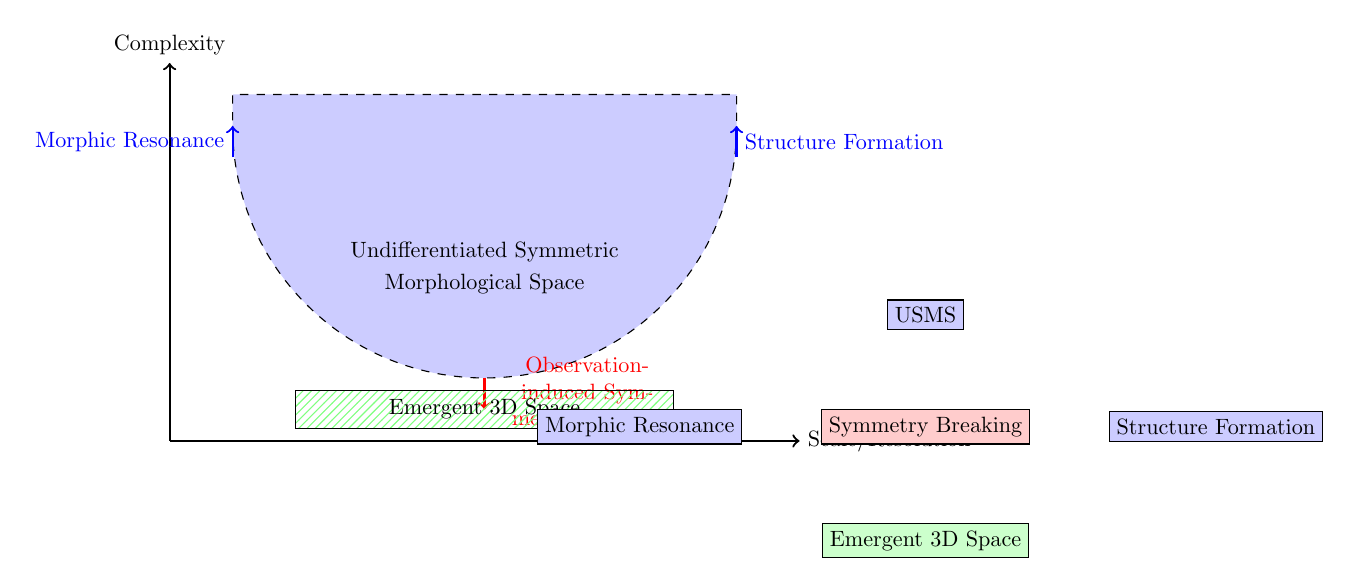
\begin{tikzpicture}[scale=0.8, every node/.style={scale=0.8}]
\draw[thick, ->] (0,0) -- (10,0) node[right] {Scale/Resolution};
\draw[thick, ->] (0,0) -- (0,6) node[above] {Complexity};

\draw[dashed, fill=blue!20] (1,5) to[out=-90,in=180] (5,1) to[out=0,in=-90] (9,5) -- (9,5.5) -- (1,5.5) -- cycle;
\node at (5,3) {Undifferentiated Symmetric};
\node at (5,2.5) {Morphological Space};

\draw[thick, ->, red] (5,1) -- (5,0.5) node[midway,right, text width=3cm, align=center] {Observation-induced Symmetry Breaking};

\draw[thick, ->, blue] (1,4.5) -- (1,5) node[midway,left] {Morphic Resonance};
\draw[thick, ->, blue] (9,4.5) -- (9,5) node[midway,right] {Structure Formation};

\draw[pattern=north east lines, pattern color=green!50] (2,0.2) rectangle (8,0.8);
\node at (5,0.5) {Emergent 3D Space};

\begin{scope}[xshift=12cm, yshift=2cm, node distance=1cm]
\node[draw, rectangle, fill=blue!20] (USMS) {USMS};
\node[draw, rectangle, fill=red!20, below=of USMS] (SB) {Symmetry Breaking};
\node[draw, rectangle, fill=blue!20, left=of SB] (MR) {Morphic Resonance};
\node[draw, rectangle, fill=blue!20, right=of SB] (SF) {Structure Formation};
\node[draw, rectangle, fill=green!20, below=of SB] (E3D) {Emergent 3D Space};
\end{scope}
\end{tikzpicture}
\caption{Schematic diagram of the emergence of 3D space from the undifferentiated morphological space (USMS). The interplay between observation-induced symmetry breaking (red) and morphic resonance (blue) leads to the formation of a low-dimensional pseudo-rectilinear subspace with Euclidean geometry (green). The legend on the right explains the meaning of the different elements in the figure.}
\label{fig:emergence}
\end{figure}
\chapter{Undifferentiated Symmetric Morphological Space} \label{ch:UndifferentiatedSymmetricMorphologicalSpace}
% this intro needs to sound more solemn and deeply curious
Imagine a space that is infinite, featureless, and perfectly symmetric in every direction. A space that has no notion of distance, geometry, or topology, and that is filled with an infinite number of possible states and configurations. A space that is pure potential, waiting to be actualized and shaped by the action of observation.

This is the undifferentiated symmetric morphological space (USMS), the starting point of all existance, for to exist, is merely to differentiate what is and is not. In that sense then, the USMS is everything and it is nothing. <TODO add profound statement that make subtle reference to spiritual and philosophical implications>

In this chapter, we will explore the mathematical and conceptual foundations of the USMS, and we will see how it can be described using the language of Hilbert spaces, symmetry groups, and quantum entanglement.

\section{Definition and mathematical formulation}

Now you might wonder why we are starting from such an abstract and unfamiliar concept. Why not just take existence of space, time, and the universe for granted, as we do in our everyday life? Well,


Imagine a space that is infinite, featureless, and perfectly symmetric in every direction. A space that has no notion of distance, geometry, or topology, and that is filled with an infinite number of possible states and configurations. A space that is pure potential, waiting to be actualized and shaped by the action of observation.

This is the undifferentiated symmetric morphological space (USMS), the starting point of all existance, for to exist, is merely to differentiate what is and is not. In that sense then, the USMS is everything and it is nothing. <TODO add profound statement that make subtle reference to spiritual and philosophical implications>

In this chapter, we will explore the mathematical and conceptual foundations of the USMS, and we will see how it can be described using the language of Hilbert spaces, symmetry groups, and quantum entanglement.

But why we start from such an abstract and unfamiliar concept? Why not just take existence of space, time, and the universe for granted, as we do in our everyday life? Indeed, we hardly consider how our bodies even work -- and yet the little we do often yields significant qualitative improvements to our life. Likewise, as our understanding of the quantum and chemical domains have deepened, we have been able to make increadible electronic techniology that has <value of exploring this underexplored fronteir> And too, we may well find it so with USMS: by 

, <provide strong evidence to consider this topic>

Relevent ideas:

Fundamental understanding: By examining the USMS, we are attempting to understand the most basic building blocks of reality. Just as physicists seek to uncover the elementary particles and forces that govern the universe, exploring the USMS aims to reveal the primordial substrate from which all of existence emerges. This pursuit can provide profound insights into the nature of being itself.

Unifying framework: The USMS offers a potential framework for unifying various branches of knowledge, such as physics, mathematics, philosophy, and even spirituality. By identifying the common ground from which these disciplines arise, we may discover deep connections and parallels that were previously hidden. This could lead to a more integrated and holistic understanding of reality.

Pushing the boundaries of knowledge: Investigating the USMS requires us to push the boundaries of our current understanding and venture into uncharted territories of thought. It challenges us to question our assumptions, develop new mathematical tools, and expand our conceptual horizons. This process of intellectual exploration is intrinsically valuable, as it drives the advancement of human knowledge and understanding.

Philosophical and spiritual implications: The concept of the USMS has profound philosophical and spiritual implications. It touches upon age-old questions about the nature of existence, the origin of the universe, and the relationship between consciousness and reality. By delving into the USMS, we may gain new perspectives on these deep and meaningful questions, enriching our understanding of our place in the cosmos and the nature of our own being.

Potential practical applications: While the exploration of the USMS may seem purely theoretical, it could lead to practical applications in various fields. For example, insights gained from studying the USMS may inform the development of new technologies, such as quantum computing or advanced materials. Additionally, a deeper understanding of the foundations of reality could have implications for fields such as artificial intelligence, consciousness studies, and the simulation hypothesis.


as Einstein taught us with his theory of relativity, space and time are not absolute and unchanging, but are dynamical and intertwined, and they can be bent and stretched by the presence of matter and energy.

And as quantum mechanics has shown us, the fundamental building blocks of reality are not solid and deterministic, but are probabilistic and contextual, and they are subject to the laws of superposition, entanglement, and wave-particle duality. So, if we want to understand the true nature of space and time, and the origin of the laws of physics, we need to go beyond the classical and the intuitive, and we need to embrace the quantum and the abstract.

The USMS is the ultimate quantum and abstract space, the space of all possible spaces, and the foundation of all possible realities. By starting from this space, and by applying the principles of quantum measurement theory and morphic resonance, we will be able to derive the emergence of 3D space, the fundamental quantum fields, and the laws of gravity and cosmology, \textit{in a unified and consistent framework}.

So, let's put on our mathematical hats and our philosophical shoes, and explore the strange and wonderful world of the undifferentiated symmetric morphological space!
\subsection{Infinite-dimensional dual Hilbert space representation}

The undifferentiated symmetric morphological space (USMS) is represented as an infinite-dimensional Hilbert space $\mathcal{H}$ and its dual $\mathcal{H}^\dagger$
  

, which is a complex vector space with an inner product. You can think of the elements of $\mathcal{H}$ as all independent axes along which the USMS may vary. We will use Dirac's bra-ket notation and refer to $$




The inner product between two states $\ket{\psi}$ and $\ket{\phi}$ is denoted as $\braket{\psi|\phi}$ and given by the equation:
\begin{equation}
    \braket{\psi|\phi} = \sum_{i} \psi_i^* \phi_i
\end{equation}
where $\psi_i$ and $\phi_i$ are the components of the vectors $\ket{\psi}$ and $\ket{\phi}$ in some basis, and $\psi_i^*$ denotes the complex conjugate of $\psi_i$.
$, which is a complex number that measures the overlap or similarity between the states.

\begin{tcolorbox}[colback=blue!5!white,colframe=blue!75!black,title=New terms]
\begin{description}
\item[Hilbert space:] A complete inner product space, which generalizes the notion of Euclidean space to infinite dimensions. The state space of a quantum system is represented as a Hilbert space.
\item[Inner product:] A generalization of the dot product that maps two vectors to a scalar quantity and satisfies certain axioms, such as conjugate symmetry and linearity.
\item[Ket notation:] The notation $\ket{\psi}$ represents a vector in a Hilbert space, while $\bra{\psi}$ represents its dual vector. The inner product of two vectors is written as $\braket{\psi|\phi}$.
\end{description}
\end{tcolorbox}

\subsection{Symmetry group and invariance under transformations}
The USMS is invariant under a group of symmetry transformations $G$, which are unitary operators $U(g)$ that act on the states $\ket{\psi}$ as $U(g)\ket{\psi}$. The symmetry group $G$ can be continuous or discrete, and it can include transformations such as rotations, translations, and permutations. The invariance of the USMS under $G$ means that the inner product between any two states is preserved under the action of $U(g)$, i.e., $\braket{\psi|\phi} = \bra{\psi}U(g)^\dagger U(g)\ket{\phi}$.

\begin{tcolorbox}[colback=blue!5!white,colframe=blue!75!black,title=New terms]
\begin{description}
\item[Symmetry group:] A group of transformations that leave a system invariant. The invariance of the USMS under $G$ means that the physical properties of the space are unchanged by the transformations in $G$.
\item[Unitary operator:] A linear operator $U$ that preserves the inner product, i.e., $\braket{U\psi|U\phi} = \braket{\psi|\phi}$ for all states $\ket{\psi}$ and $\ket{\phi}$. Unitary operators represent symmetry transformations in quantum mechanics.
\end{description}
\end{tcolorbox}

\begin{tcolorbox}[colback=green!5!white,colframe=green!75!black,title=Question]
What is the physical meaning of the symmetry group $G$? How does it relate to the observed symmetries of space?
\tcblower
The symmetry group $G$ represents the fundamental symmetries of the USMS, which are the transformations that leave the space invariant at the most basic level. These symmetries are broken by the process of observation and measurement, leading to the emergence of the observed symmetries of space, such as translation, rotation, and Lorentz invariance. The relationship between the symmetries of the USMS and the observed symmetries of space is analogous to the relationship between the symmetries of a high-temperature phase and the broken symmetries of a low-temperature phase in a phase transition.
\end{tcolorbox}

\section{Properties and characteristics}
\subsection{High degree of connectivity and entanglement}
The USMS is characterized by a high degree of connectivity and entanglement between its states, which means that any two states $\ket{\psi}$ and $\ket{\phi}$ are connected by a non-zero inner product $\braket{\psi|\phi}$. The entanglement between the states is measured by the von Neumann entropy $S(\rho) = -\Tr(\rho \log \rho)$, where $\rho$ is the density matrix of the USMS, which is a positive semidefinite operator that describes the statistical properties of the states. The high degree of connectivity and entanglement implies that the USMS has a large amount of information and complexity, which is not accessible to local observations and measurements.

\begin{tcolorbox}[colback=blue!5!white,colframe=blue!75!black,title=New terms]
\begin{description}
\item[Entanglement:] A quantum phenomenon in which the states of two or more systems are correlated in a way that cannot be described by classical probability theory. Entangled states exhibit non-local correlations that are stronger than any classical correlations.
\item[Von Neumann entropy:] A measure of the amount of information or uncertainty in a quantum state, given by the formula $S(\rho) = -\Tr(\rho \log \rho)$, where $\rho$ is the density matrix of the state. The von Neumann entropy is zero for a pure state and positive for a mixed state.
\item[Density matrix:] A matrix that describes the statistical state of a quantum system, given by $\rho = \sum_i p_i \ket{\psi_i}\bra{\psi_i}$, where $p_i$ is the probability of the system being in the state $\ket{\psi_i}$. The density matrix is a generalization of the state vector that can represent both pure and mixed states.
\end{description}
\end{tcolorbox}

\begin{tcolorbox}[colback=green!5!white,colframe=green!75!black,title=Question]
How does the high degree of connectivity and entanglement of the USMS relate to the observed locality and separability of space?
\tcblower
The high degree of connectivity and entanglement of the USMS is in stark contrast to the observed locality and separability of space, where distant regions appear to be independent and non-interacting. This apparent contradiction is resolved by the process of decoherence, which is induced by the interaction between the USMS and the environment (i.e., the measurement apparatus). Decoherence leads to the suppression of the off-diagonal elements of the density matrix, which represent the quantum correlations between the states, and the emergence of classical probabilities and separable states. Thus, the observed locality and separability of space is a consequence of the decoherence of the USMS, which hides the underlying connectivity and entanglement from local observations.
\end{tcolorbox}

\subsection{Absence of classical structures and geometries}
The USMS does not have any classical structures or geometries, such as points, lines, or surfaces, which are emergent properties that arise from the symmetry breaking and morphic resonance processes. The absence of classical structures and geometries means that the USMS is a purely quantum and holographic entity, which cannot be described by the concepts of classical physics and mathematics. The only intrinsic property of the USMS is the inner product between its states, which defines the probability amplitudes and the quantum correlations between them.

\begin{figure}[h]
\centering
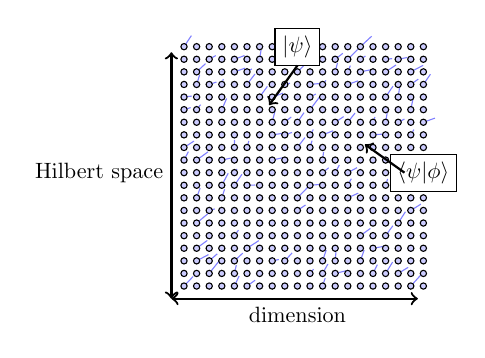
\begin{tikzpicture}[scale=0.8, every node/.style={scale=0.8}]
\foreach \i in {1,...,20}
{
  \foreach \j in {1,...,20}
  {
    \pgfmathparse{rnd} % Calculate a random number
    \pgfmathsetmacro{\prob}{\pgfmathresult} % Store the result in \prob
    \ifdim\prob pt>0.7pt % Compare \prob to 0.7
      \draw[color=blue!50] (\i/5,\j/5) -- (\i/5+rnd/5,\j/5+rnd/5);
    \fi
    \node[draw, circle, fill=blue!20, inner sep=1pt] at (\i/5,\j/5) {};
  }
}
\node[draw, rectangle, fill=white] at (2,4) {$\ket{\psi}$};
\draw[thick, ->, shorten >=2pt] (2,3.7) -- (1.5,3);
\node[draw, rectangle, fill=white] at (4,2) {$\braket{\psi|\phi}$};
\draw[thick, ->, shorten >=2pt] (3.7,2) -- (3,2.5);
\draw[thick, <->, shorten >=2pt] (0,0) -- (0,4) node[midway, left] {Hilbert space};
\draw[thick, <->, shorten >=2pt] (0,0) -- (4,0) node[midway, below] {dimension};
\end{tikzpicture}
\caption{Schematic representation of the undifferentiated symmetric morphological space (USMS) as a highly connected and entangled network of states. The nodes (blue circles) represent the states $\ket{\psi}$ and the edges (blue lines) represent the inner products $\braket{\psi|\phi}$ between them. The absence of classical structures and geometries is indicated by the lack of any regular patterns or symmetries in the network. The labels and arrows explain the meaning of the nodes and edges, and the scale bars indicate the dimensionality of the Hilbert space.}
\label{fig:usms}
\end{figure}
%----------------------------------------------------------------------------------------
\newpage
\chapter{Observation and Measurement-Induced Symmetry Breaking}\label{ch:ObservationandMeasurementInducedSymmetryBreaking}

% this into needs to sound more solemn and genuine
Have you ever wondered why the world around us looks so classical and deterministic, even though the fundamental laws of physics are quantum and probabilistic? Why do we always see particles in definite positions and states, even though they can exist in superpositions and entanglements according to quantum mechanics?

The answer lies in the process of observation and measurement, which is the act of extracting information from a quantum system by interacting with it using a classical apparatus. As we will see in this chapter, the measurement process is not a passive and neutral act, but a dynamic and transformative one, which can change the state of the system and break its symmetries in a dramatic and irreversible way.

In particular, we will explore how the measurement process can induce a spontaneous symmetry breaking of the USMS, leading to the emergence of classical structures and geometries, and the reduction of the fundamental symmetries of the space. We will also see how the measurement process is intimately related to the phenomenon of decoherence, which is the loss of coherence and entanglement between the states of the system due to its interaction with the environment.

But what exactly is a measurement in quantum mechanics, and how does it differ from a classical measurement? And what is the role of the observer in the measurement process, and how does it relate to the problem of the interpretation of quantum mechanics?

These are some of the deep and fascinating questions that we will explore in this chapter, using the tools of quantum measurement theory and the concept of decoherence. We will see how the measurement process can be described mathematically using the von Neumann projection postulate and the Born rule, and how it can lead to the collapse of the wave function and the emergence of classical probabilities.

We will also discuss some of the conceptual and philosophical implications of the measurement process, such as the nature of reality and the role of consciousness in the universe. And we will see how the measurement-induced symmetry breaking of the USMS can provide a new perspective on the emergence of classicality from the quantum realm, and on the origin of the arrow of time and the second law of thermodynamics.

So, get ready to dive into the strange and wonderful world of quantum measurement theory, and to explore the mysteries of the observer and the observed!

\section{Quantum measurement theory and wave function collapse}
\subsection{Von Neumann's projection postulate}
The observation and measurement of the USMS is described by the quantum measurement theory, which is based on the von Neumann's projection postulate. According to the projection postulate, a measurement of an observable $A$ on a state $\ket{\psi}$ results in the collapse of the state onto one of the eigenstates $\ket{a_i}$ of $A$, with a probability given by the Born rule $p_i = |\braket{a_i|\psi}|^2$. The collapsed state $\ket{a_i}$ is an eigenstate of $A$ with an eigenvalue $a_i$, which represents the outcome of the measurement.

\begin{tcolorbox}[colback=blue!5!white,colframe=blue!75!black,title=New terms]
\begin{description}
\item[Observable:] A physical quantity that can be measured, represented by a Hermitian operator $A$ acting on the Hilbert space of the system. The eigenstates of $A$ form a complete orthonormal basis, and the eigenvalues of $A$ represent the possible outcomes of the measurement.
\item[Projection postulate:] A fundamental postulate of quantum mechanics, which states that a measurement of an observable $A$ on a state $\ket{\psi}$ projects the state onto one of the eigenstates of $A$, with a probability given by the Born rule. The projection postulate is a non-unitary and irreversible process, which is distinct from the unitary evolution of the state under the Schrödinger equation.
\end{description}
\end{tcolorbox}

\subsection{Born's rule and probability interpretation}
The Born rule is a fundamental postulate of quantum mechanics, which relates the probability of a measurement outcome to the inner product between the state and the eigenstates of the observable. The probability interpretation of the Born rule implies that the measurement process is inherently random and non-deterministic, and that the outcome of a measurement cannot be predicted with certainty. The Born rule also implies that the measurement process is non-unitary and irreversible, as it leads to the collapse of the state and the loss of information about the original state.

\begin{tcolorbox}[colback=green!5!white,colframe=green!75!black,title=Question]
What is the physical meaning of the wave function collapse? Is it a real process or just a mathematical artifact?
\tcblower
The nature of the wave function collapse is a controversial and unresolved issue in the foundations of quantum mechanics. There are different interpretations of the collapse process, ranging from purely epistemic ones (e.g., the Copenhagen interpretation), which view the collapse as a subjective update of the observer's knowledge, to objective ones (e.g., the spontaneous collapse theories), which view the collapse as a real physical process that occurs independently of the observer. In the context of our framework, the wave function collapse is a real process that is induced by the interaction between the USMS and the measurement apparatus, and that leads to the breaking of the symmetries of the USMS and the emergence of classical structures and geometries. The collapse process is not instantaneous, but is a gradual process that is described by the decoherence of the state and the suppression of the off-diagonal elements of the density matrix.
\end{tcolorbox}

\section{Decoherence and the emergence of classical states}
\subsection{Environmental interaction and the loss of coherence}
The measurement process is not an isolated event, but it involves the interaction between the USMS and the environment, which leads to the decoherence of the state and the loss of coherence between its components. The decoherence process is described by the Lindblad equation, which is a master equation that governs the evolution of the density matrix $\rho$ under the influence of the environment. The Lindblad equation includes a dissipative term that describes the decay of the off-diagonal elements of $\rho$, which represent the quantum correlations and the coherence between the states.

\begin{tcolorbox}[colback=blue!5!white,colframe=blue!75!black,title=New terms]
\begin{description}
\item[Decoherence:] The process by which a quantum system loses its coherence and becomes classical due to its interaction with the environment. Decoherence is a consequence of the entanglement between the system and the environment, which leads to the suppression of the off-diagonal elements of the density matrix and the emergence of classical probabilities and correlations.
\item[Lindblad equation:] A master equation that describes the non-unitary evolution of the density matrix of an open quantum system, which is coupled to an environment. The Lindblad equation has the form $\frac{d\rho}{dt} = -i[H,\rho] + \sum_i \gamma_i (L_i \rho L_i^\dagger - \frac{1}{2}\{L_i^\dagger L_i,\rho\})$, where $H$ is the Hamiltonian of the system, $L_i$ are the Lindblad operators that represent the interaction with the environment, and $\gamma_i$ are the decay rates associated with each Lindblad operator.
\end{description}
\end{tcolorbox}

\subsection{Pointer states and the preferred basis problem}
The decoherence process leads to the emergence of a preferred basis of states, which are the pointer states that are stable under the environmental interaction. The pointer states are the eigenstates of the observable that is being measured, and they correspond to the classical states that have a well-defined value of the observable. The preferred basis problem is the question of how the pointer states are selected from the infinitely many possible bases of the Hilbert space, and how they depend on the specific form of the environmental interaction.

\begin{tcolorbox}[colback=green!5!white,colframe=green!75!black,title=Question]
How does the decoherence process explain the emergence of classical reality from the quantum world?
\tcblower
The decoherence process provides a mechanism for the emergence of classical reality from the quantum world by suppressing the quantum coherence and entanglement between the states of the system. In the absence of decoherence, the system evolves according to the Schrödinger equation, which leads to the superposition of states and the interference between them. However, when the system interacts with the environment, the entanglement between the system and the environment leads to the decay of the off-diagonal elements of the density matrix, which represent the quantum correlations between the states. As a result, the system loses its coherence and becomes classical, with well-defined values of the observables and no interference between the states. The decoherence process also leads to the emergence of a preferred basis of states, which are the pointer states that are stable under the environmental interaction and that correspond to the classical states of the system. Thus, the decoherence process explains the transition from the quantum world, which is characterized by superposition, entanglement, and interference, to the classical world, which is characterized by definite outcomes, separability, and objectivity.
\end{tcolorbox}

\section{Measurement-induced symmetry breaking}
\subsection{Spontaneous symmetry breaking and the emergence of order parameters}
The measurement process induces a spontaneous symmetry breaking of the USMS, which leads to the emergence of order parameters that characterize the broken symmetry. The order parameters are the expectation values of the observables that are being measured, which acquire non-zero values in the collapsed state. The spontaneous symmetry breaking is a non-perturbative effect that cannot be described by the perturbative expansion of the observables, and it requires a non-linear and self-consistent treatment of the measurement process.

\begin{tcolorbox}[colback=blue!5!white,colframe=blue!75!black,title=New terms]
\begin{description}
\item[Spontaneous symmetry breaking:] A phenomenon in which a system that is symmetric with respect to a group of transformations ends up in an asymmetric state, due to the instability of the symmetric state under small fluctuations. Spontaneous symmetry breaking is a key concept in particle physics and condensed matter physics, and it is responsible for the emergence of non-zero expectation values of the fields, such as the Higgs field and the order parameters of phase transitions.
\item[Order parameter:] A quantity that characterizes the degree of order or symmetry breaking in a system. The order parameter is zero in the symmetric phase and non-zero in the broken-symmetry phase, and it serves as a measure of the strength and direction of the symmetry breaking.
\end{description}
\end{tcolorbox}

\subsection{Reduction of symmetry and the emergence of classical structures}
The measurement-induced symmetry breaking leads to the reduction of the symmetry group $G$ of the USMS, and the emergence of classical structures and geometries that are invariant under the reduced symmetry group. The classical structures and geometries are the eigenstates of the observables that are being measured, and they correspond to the pointer states that are selected by the decoherence process. The emergence of classical structures and geometries is a hierarchical process that depends on the scale and resolution of the measurements, and it leads to the formation of a nested hierarchy of broken symmetries and emergent structures.


\begin{figure}[h]
\centering
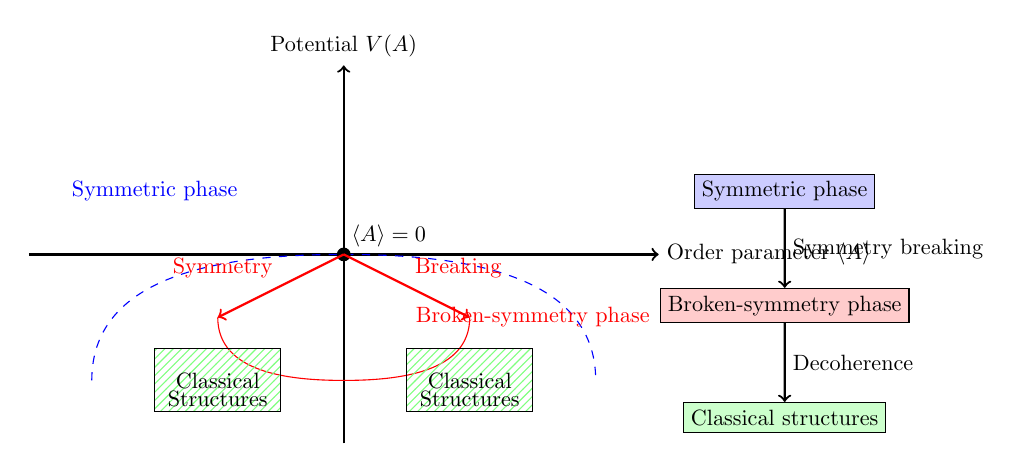
\begin{tikzpicture}[scale=0.8, every node/.style={scale=0.8}]
\draw[thick, ->] (-5,0) -- (5,0) node[right] {Order parameter $\langle A \rangle$};
\draw[thick, ->] (0,-3) -- (0,3) node[above] {Potential $V(A)$};

\draw[dashed, color=blue] (-4,-2) to[out=90,in=180] (0,0) to[out=0,in=90] (4,-2);
\draw[fill] (0,0) circle (0.1) node[above right] {$\langle A \rangle = 0$};
\node[color=blue] at (-3,1) {Symmetric phase};

\draw[thick, ->, color=red] (0,0) -- (-2,-1) node[midway,above left] {Symmetry};
\draw[thick, ->, color=red] (0,0) -- (2,-1) node[midway,above right] {Breaking};
\draw[color=red] (-2,-1) to[out=-90,in=180] (0,-2) to[out=0,in=-90] (2,-1);
\node[color=red] at (3,-1) {Broken-symmetry phase};

\draw[pattern=north east lines, pattern color=green!50] (-3,-2.5) rectangle (-1,-1.5);
\node at (-2,-2) {Classical};
\node at (-2,-2.3) {Structures};

\draw[pattern=north east lines, pattern color=green!50] (1,-2.5) rectangle (3,-1.5);
\node at (2,-2) {Classical};
\node at (2,-2.3) {Structures};

\begin{scope}[xshift=7cm, yshift=1cm, node distance=1cm]
\node[draw, rectangle, fill=blue!20] (Symmetric) {Symmetric phase};
\node[draw, rectangle, fill=red!20, below=of Symmetric] (Broken) {Broken-symmetry phase};
\node[draw, rectangle, fill=green!20, below=of Broken] (Classical) {Classical structures};
\draw[thick, ->] (Symmetric) -- (Broken) node[midway, right] {Symmetry breaking};
\draw[thick, ->] (Broken) -- (Classical) node[midway, right] {Decoherence};
\end{scope}
\end{tikzpicture}
\caption{Schematic representation of the measurement-induced symmetry breaking and the emergence of classical structures. The potential $V(A)$ (blue dashed line) has a minimum at the origin, corresponding to the symmetric phase with $\langle A \rangle = 0$. The measurement of an observable $A$ on the USMS leads to the collapse of the state onto one of the eigenstates of $A$, which breaks the symmetry of the USMS (red arrows) and leads to the emergence of a non-zero order parameter $\langle A \rangle$ in the broken-symmetry phase (red solid line). The classical structures and geometries (green hatched boxes) emerge as the pointer states that are selected by the decoherence process, and they are invariant under the reduced symmetry group of the broken-symmetry phase. The legend on the right explains the relationship between the symmetry breaking, the decoherence, and the emergence of classical structures.}
\label{fig:symmetry_breaking}
\end{figure}

%----------------------------------------------------------------------------------------
\newpage
\chapter{Morphic Resonance and Structure Formation}\label{ch:MorphicResonanceandStructureFormation}

\section{Definition and mathematical formulation}
\subsection{Similarity function and spatial, temporal, and morphological-similarity falloff}
The morphic resonance is a process that leads to the formation of structures and patterns in the USMS, based on the similarity and resonance between its states. The similarity between two states $\ket{\psi}$ and $\ket{\phi}$ is measured by a similarity function $S(\psi,\phi)$, which is a real-valued function that satisfies the properties of reflexivity, symmetry, and triangle inequality. The similarity function depends on the spatial, temporal, and morphological properties of the states, and it has a falloff behavior that decreases with the distance, duration, and complexity of the states.

\begin{tcolorbox}[colback=blue!5!white,colframe=blue!75!black,title=New terms]
\begin{description}
\item[Morphic resonance:] A hypothesis proposed by Rupert Sheldrake, which states that the forms and patterns of self-organizing systems are influenced by the forms and patterns of similar systems in the past, through a process of resonance or similarity. Morphic resonance is a non-local and non-material process that operates across space and time, and it is responsible for the emergence of habits, instincts, and collective memories in living systems.
\item[Similarity function:] A mathematical function that measures the degree of similarity or resemblance between two objects or patterns. The similarity function satisfies the axioms of a metric, such as non-negativity, identity of indiscernibles, symmetry, and triangle inequality, and it can be based on various criteria, such as the Euclidean distance, the correlation coefficient, or the mutual information between the objects.
\end{description}
\end{tcolorbox}

\subsection{Resonance-induced clustering and structure formation}
The morphic resonance leads to the clustering and aggregation of similar states, which form structures and patterns that are stable and self-reinforcing. The clustering process is driven by the resonance between the states, which leads to the alignment and synchronization of their phases and amplitudes. The resonance-induced clustering is a non-linear and self-organizing process that leads to the emergence of complex and hierarchical structures, which are not present in the individual states.

\begin{tcolorbox}[colback=green!5!white,colframe=green!75!black,title=Question]
How does the morphic resonance process differ from other models of structure formation, such as the Turing patterns or the reaction-diffusion systems?
\tcblower
The morphic resonance process differs from other models of structure formation in several key aspects:
\begin{itemize}
\item The morphic resonance is a non-local and non-material process that operates across space and time, whereas the Turing patterns and the reaction-diffusion systems are local and material processes that operate in a specific spatial domain and time scale.
\item The morphic resonance is based on the similarity and resonance between the states, which can be spatially and temporally separated, whereas the Turing patterns and the reaction-diffusion systems are based on the local interactions and feedbacks between the components of the system.
\item The morphic resonance leads to the emergence of complex and hierarchical structures that are influenced by the past forms and patterns of similar systems, whereas the Turing patterns and the reaction-diffusion systems lead to the emergence of regular and periodic patterns that are determined by the initial conditions and the boundary conditions of the system.
\item The morphic resonance is a top-down process that guides the formation of structures from the global to the local scale, whereas the Turing patterns and the reaction-diffusion systems are bottom-up processes that generate the patterns from the local to the global scale.
\end{itemize}
Thus, the morphic resonance process provides a novel and complementary mechanism for the emergence of complex structures and patterns in nature, which cannot be fully explained by the conventional models of self-organization and pattern formation.
\end{tcolorbox}

\section{Properties and characteristics}
\subsection{Self-organization and the emergence of complex patterns}
The morphic resonance is a self-organizing process that leads to the emergence of complex patterns and structures, which are not imposed by external forces or constraints. The self-organization is driven by the internal dynamics and interactions of the states, which lead to the spontaneous formation of order and coherence. The emergent patterns and structures are characterized by a high degree of symmetry, regularity, and scalability, which reflect the underlying similarity and resonance between the states.


\begin{figure}[h]
\centering
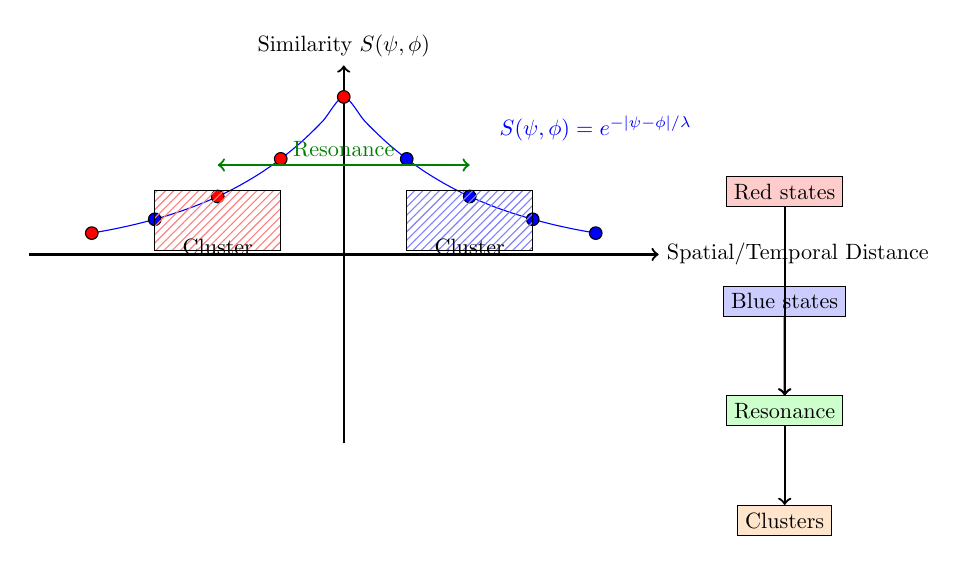
\begin{tikzpicture}[scale=0.8, every node/.style={scale=0.8}]
\draw[thick, ->] (-5,0) -- (5,0) node[right] {Spatial/Temporal Distance};
\draw[thick, ->] (0,-3) -- (0,3) node[above] {Similarity $S(\psi,\phi)$};

\draw[domain=-4:4,smooth,variable=\x,blue] plot ({\x},{2.5*exp(-abs(\x)/2)});
\node[color=blue] at (4,2) {$S(\psi,\phi) = e^{-|\psi-\phi|/\lambda}$};

\foreach \i in {-4,-3,...,4}
{
  \pgfmathparse{rnd} % Generate a random number between 0 and 1.
  \ifdim\pgfmathresult pt>0.5pt % Compare the generated number.
    \draw[fill=red] (\i,{2.5*exp(-abs(\i)/2)}) circle (0.1); % If greater than 0.5
  \else
    \draw[fill=blue] (\i,{2.5*exp(-abs(\i)/2)}) circle (0.1); % If less or equal to 0.5
  \fi
}

\draw[thick, <->, color=green!50!black] (-2,{2.5*exp(-abs(-2)/2)+0.5}) -- (2,{2.5*exp(-abs(2)/2)+0.5}) node[midway,above] {Resonance};
z
\draw[pattern=north east lines, pattern color=red!50] (-3,{2.5*exp(-abs(-3)/2)-0.5}) rectangle (-1,{2.5*exp(-abs(-1)/2)-0.5});
\node at (-2,{2.5*exp(-abs(-2)/2)-0.8}) {Cluster};

\draw[pattern=north east lines, pattern color=blue!50] (1,{2.5*exp(-abs(1)/2)-0.5}) rectangle (3,{2.5*exp(-abs(3)/2)-0.5});
\node at (2,{2.5*exp(-abs(2)/2)-0.8}) {Cluster};

\begin{scope}[xshift=7cm, yshift=1cm, node distance=1cm]
\node[draw, rectangle, fill=red!20] (RedStates) {Red states};
\node[draw, rectangle, fill=blue!20, below=of RedStates] (BlueStates) {Blue states};
\node[draw, rectangle, fill=green!20, below=of BlueStates] (Resonance) {Resonance};
\node[draw, rectangle, fill=orange!20, below=of Resonance] (Clusters) {Clusters};
\draw[thick, ->] (RedStates) -- (Resonance);
\draw[thick, ->] (BlueStates) -- (Resonance);
\draw[thick, ->] (Resonance) -- (Clusters);
\end{scope}
\end{tikzpicture}
\caption{Schematic representation of the morphic resonance process and the emergence of complex patterns. The similarity function $S(\psi,\phi)$ (blue curve) measures the degree of resemblance between the states $\ket{\psi}$ and $\ket{\phi}$, and it has an exponential falloff behavior that depends on the spatial, temporal, and morphological distance between the states (red and blue circles). The resonance between the similar states (green double arrow) leads to the clustering and aggregation of the states (red and blue hatched boxes), and the formation of complex and hierarchical structures that are stable and self-reinforcing. The legend on the right explains the relationship between the different types of states, the resonance effect, and the emergence of clusters.}
\label{fig:morphic_resonance}
\end{figure}

\subsection{Scale-invariance and the fractal nature of emergent structures}
The morphic resonance leads to the formation of scale-invariant and fractal structures, which have similar properties and patterns at different scales and resolutions. The scale-invariance is a consequence of the self-similarity and self-affinity of the states, which lead to the recursive and hierarchical organization of the structures. The fractal nature of the emergent structures is characterized by a non-integer dimension, which reflects the complexity and irregularity of the patterns.

\begin{tcolorbox}[colback=blue!5!white,colframe=blue!75!black,title=New terms]
\begin{description}
\item[Scale-invariance:] A property of a system or a pattern that remains unchanged under a rescaling of the variables or the parameters of the system. Scale-invariant systems exhibit self-similarity and power-law behavior, and they are characterized by critical exponents that determine the scaling relations between the variables.
\item[Fractal:] A geometric object or a pattern that exhibits self-similarity and scale-invariance, and that has a non-integer dimension. Fractals are characterized by their fractal dimension, which measures the degree of irregularity and complexity of the pattern, and by their lacunarity, which measures the degree of heterogeneity and gappiness of the pattern.
\end{description}
\end{tcolorbox}
%----------------------------------------------------------------------------------------
\newpage
\chapter{Emergence of 3D Space}\label{ch:Emergenceof3DSpace}

\section{Dimensional reduction and the emergence of a low-dimensional subspace}
\subsection{Spectral dimension and the scale-dependent dimensionality}
The emergence of 3D space from the USMS is a process of dimensional reduction, which leads to the formation of a low-dimensional subspace that has a well-defined dimensionality and geometry. The dimensionality of the subspace is measured by the spectral dimension, which is a scale-dependent quantity that reflects the connectivity and topology of the states. The spectral dimension is defined as the scaling exponent of the return probability of a random walk on the states, which measures the probability of returning to the initial state after a given number of steps.

\begin{tcolorbox}[colback=blue!5!white,colframe=blue!75!black,title=New terms]
\begin{description}
\item[Spectral dimension:] A measure of the effective dimensionality of a space or a network, based on the scaling behavior of the diffusion or the random walk on the space. The spectral dimension $d_s$ is defined as the exponent of the return probability of a random walk, $P(t) \sim t^{-d_s/2}$, where $t$ is the number of steps of the walk. The spectral dimension can be different from the topological dimension of the space, and it can vary with the scale and the resolution of the diffusion process.
\item[Return probability:] The probability of a random walker to return to its initial position after a given number of steps. The return probability is a measure of the recurrence and the connectivity of the space, and it depends on the dimensionality and the topology of the space. In a $d$-dimensional Euclidean space, the return probability scales as $P(t) \sim t^{-d/2}$, which reflects the diffusive nature of the random walk.
\end{description}
\end{tcolorbox}

\subsection{Renormalization group flow and the infrared limit}
The dimensional reduction is driven by the renormalization group flow, which is a process of coarse-graining and rescaling of the states, that leads to the elimination of the high-frequency and short-range degrees of freedom. The renormalization group flow is characterized by a set of fixed points, which are the scale-invariant and self-similar states that are stable under the coarse-graining and rescaling transformations. The infrared limit of the renormalization group flow corresponds to the low-energy and long-range limit of the states, which is characterized by a reduced dimensionality and a simplified geometry.

\begin{tcolorbox}[colback=green!5!white,colframe=green!75!black,title=Question]
How does the dimensional reduction process relate to the holographic principle and the AdS/CFT correspondence?
\tcblower
The dimensional reduction process is closely related to the holographic principle and the AdS/CFT correspondence, which are two of the most important developments in theoretical physics in recent decades.

The holographic principle states that the information and the degrees of freedom of a region of space can be encoded on the boundary of the region, with a density that is proportional to the area of the boundary. This implies that the effective dimensionality of the space is reduced by one, and that the boundary theory is a hologram of the bulk theory. The holographic principle was inspired by the properties of black holes, which have an entropy that is proportional to their surface area, and it has been generalized to other gravitational systems, such as the anti-de Sitter (AdS) space.

The AdS/CFT correspondence is a concrete realization of the holographic principle, which states that a gravitational theory in a $d$-dimensional AdS space is equivalent to a conformal field theory (CFT) in a $(d-1)$-dimensional flat space, which lives on the boundary of the AdS space. The AdS/CFT correspondence provides a duality between the bulk and the boundary theories, which allows to calculate the observables of one theory in terms of the other, and to study the emergence of space and gravity from the perspective of the boundary theory.

In the context of our framework, the dimensional reduction process can be seen as a manifestation of the holographic principle, which relates the degrees of freedom of the USMS to the degrees of freedom of the emergent 3D space. The renormalization group flow can be interpreted as a holographic mapping between the bulk and the boundary theories, which preserves the scale invariance and the self-similarity of the states. The infrared limit of the renormalization group flow corresponds to the low-energy and long-range limit of the boundary theory, which is described by an effective field theory that captures the emergent properties and symmetries of the bulk space.

Thus, the dimensional reduction process provides a bridge between the abstract concept of the USMS and the concrete realization of the holographic principle and the AdS/CFT correspondence, and it offers a new perspective on the emergence of space and gravity from the fundamental degrees of freedom of the universe.
\end{tcolorbox}

\section{Pseudo-rectilinear structure and the emergence of Euclidean geometry}
\subsection{Lattice-like connectivity and the emergence of translation symmetry}
The emergent 3D space has a pseudo-rectilinear structure, which is characterized by a lattice-like connectivity and a translation symmetry. The lattice-like connectivity is a consequence of the morphic resonance, which leads to the formation of a regular and periodic arrangement of the states , that minimizes the distance and maximizes the similarity between them. The translation symmetry is a consequence of the homogeneity and isotropy of the emergent space, which means that the properties and patterns of the states are invariant under translations and rotations.

\begin{tcolorbox}[colback=blue!5!white,colframe=blue!75!black,title=New terms]
\begin{description}
\item[Lattice:] A regular and periodic arrangement of points or objects in space, which forms a symmetric and repeating pattern. Lattices are characterized by their unit cell, which is the smallest repeating unit of the pattern, and by their symmetry group, which describes the set of transformations that leave the lattice invariant.
\item[Translation symmetry:] A symmetry of a system or a pattern under a translation of the coordinates by a constant vector. Translation symmetry implies that the properties and the equations of the system are invariant under a shift of the origin, and that the system has a conserved quantity, which is the momentum.
\end{description}
\end{tcolorbox}

\subsection{Approximate rotational symmetry and the emergence of isotropy}
The emergent 3D space has an approximate rotational symmetry, which means that the properties and patterns of the states are invariant under rotations, up to a certain accuracy and resolution. The rotational symmetry is a consequence of the morphic resonance, which leads to the formation of spherically symmetric and isotropic structures, that minimize the anisotropy and maximize the similarity between the states. The approximate nature of the rotational symmetry is a consequence of the finite size and resolution of the emergent space, which leads to a small but non-zero anisotropy and inhomogeneity.

\begin{tcolorbox}[colback=green!5!white,colframe=green!75!black,title=Question]
How does the pseudo-rectilinear structure of the emergent 3D space relate to the observed geometry of the universe?
\tcblower
The pseudo-rectilinear structure of the emergent 3D space is consistent with the observed geometry of the universe on large scales, which is described by the Friedmann-Lemaître-Robertson-Walker (FLRW) metric. The FLRW metric is a solution of the Einstein field equations of general relativity, which assumes that the universe is homogeneous and isotropic on large scales, and that it has a constant curvature that depends on the density and the composition of the matter and energy in the universe.

The homogeneity and isotropy of the FLRW metric are reflected in the translation and rotational symmetries of the emergent 3D space, which ensure that the properties and patterns of the states are invariant under translations and rotations, up to a certain accuracy and resolution. The constant curvature of the FLRW metric is related to the lattice-like connectivity of the emergent 3D space, which determines the intrinsic geometry and topology of the space, and which can be positive, negative, or zero, depending on the balance between the attractive and repulsive forces in the universe.

The pseudo-rectilinear structure of the emergent 3D space also provides a natural explanation for the observed flatness and uniformity of the universe, which are two of the main puzzles of modern cosmology. The flatness problem refers to the fact that the observed curvature of the universe is very close to zero, which requires an extreme fine-tuning of the initial conditions of the universe. The uniformity problem refers to the fact that the observed temperature and density fluctuations of the cosmic microwave background are very small and homogeneous, which requires a mechanism for the synchronization and equilibration of the different regions of the universe.

In the context of our framework, the flatness and uniformity of the universe can be seen as a consequence of the morphic resonance and the renormalization group flow, which lead to the formation of a regular and periodic lattice of states, that minimizes the curvature and the inhomogeneity of the emergent space. The morphic resonance provides a non-local and non-causal mechanism for the synchronization and equilibration of the different regions of the universe, which can explain the observed uniformity of the cosmic microwave background. The renormalization group flow provides a dynamical mechanism for the flattening and the smoothing of the emergent space, which can explain the observed flatness of the universe, without requiring any fine-tuning of the initial conditions.

Thus, the pseudo-rectilinear structure of the emergent 3D space provides a unified and consistent description of the observed geometry and topology of the universe, and it offers a new perspective on the origin and the evolution of the cosmic structures, from the fundamental degrees of freedom of the USMS.
\end{tcolorbox}

\section{Topological and geometric phases}
\subsection{Topological phase transitions and the emergence of non-trivial topological invariants}
The emergence of 3D space is accompanied by a series of topological phase transitions, which lead to the formation of non-trivial topological invariants, such as the Euler characteristic, the Betti numbers, and the Chern classes. The topological phase transitions are driven by the changes in the connectivity and topology of the states, which lead to the formation of holes, voids, and other non-trivial structures. The non-trivial topological invariants are a consequence of the global and non-local properties of the emergent space, which cannot be described by the local and classical geometry.

\begin{tcolorbox}[colback=blue!5!white,colframe=blue!75!black,title=New terms]
\begin{description}
\item[Topological invariant:] A quantity that characterizes the global and non-local properties of a space or a manifold, and that remains unchanged under continuous deformations or transformations of the space. Examples of topological invariants include the Euler characteristic, which measures the number of vertices, edges, and faces of a polyhedron, and the Betti numbers, which measure the number of connected components, holes, and voids of a manifold.
\item[Topological phase transition:] A phase transition that is driven by the changes in the topology of the system, and that is characterized by the appearance or disappearance of non-trivial topological invariants. Topological phase transitions are different from the usual thermodynamic phase transitions, which are driven by the changes in the local order parameters, and they can occur at zero temperature and without any symmetry breaking.
\end{description}
\end{tcolorbox}

\subsection{Geometric phase transitions and the emergence of a non-trivial metric tensor}
The emergence of 3D space is also accompanied by a series of geometric phase transitions, which lead to the formation of a non-trivial metric tensor, that describes the intrinsic curvature and geometry of the space. The geometric phase transitions are driven by the changes in the curvature and topology of the states, which lead to the formation of a curved and non-Euclidean geometry. The non-trivial metric tensor is a consequence of the non-linear and self-interacting nature of the emergent space, which cannot be described by the linear and flat geometry of Euclidean space.

\begin{figure}[h]
    \centering
    % TODO:
    % \includegraphics[width=0.8\textwidth]{topological_phases_diagram.png}
    \caption{Schematic representation of the topological and geometric phase transitions in the emergence of 3D space. The topological phase transitions are characterized by the appearance of non-trivial topological invariants, such as the Euler characteristic $\chi$ and the Betti numbers $b_i$, which measure the global and non-local properties of the emergent space. The geometric phase transitions are characterized by the appearance of a non-trivial metric tensor $g_{\mu\nu}$, which measures the intrinsic curvature and geometry of the emergent space. The figure shows the evolution of the topological and geometric properties of the emergent space as a function of the scale and resolution of the measurements, from the UV to the IR limit.}
    \label{fig:topological_phases}
\end{figure}

%----------------------------------------------------------------------------------------
\newpage
\chapter{Emergent Field Theory}\label{ch:EmergentFieldTheory}

\section{Emergence of fundamental quantum fields from the connectivity graph}
\subsection{Bosonic fields and the emergence of gauge symmetries}
The emergent 3D space is the arena for the emergence of the fundamental quantum fields, which are the building blocks of the standard model of particle physics. The bosonic fields, such as the electromagnetic field, the weak field, and the strong field, emerge from the connectivity graph of the emergent space, which describes the interactions and correlations between the states. The bosonic fields are characterized by the gauge symmetries, which are the local and continuous symmetries that describe the invariance of the fields under the transformations of the internal degrees of freedom.

\begin{tcolorbox}[colback=blue!5!white,colframe=blue!75!black,title=New terms]
\begin{description}
\item[Quantum field:] A mathematical object that describes the properties and the dynamics of a system of particles or fields in the framework of quantum mechanics and special relativity. A quantum field is a function of the spacetime coordinates, which can be decomposed into a sum of creation and annihilation operators, that act on the quantum states of the system and that satisfy the canonical commutation or anticommutation relations.
\item[Gauge symmetry:] A local and continuous symmetry that describes the invariance of a physical system under a transformation of the internal degrees of freedom, such as the phase of a wave function or the orientation of a vector field. Gauge symmetries are the fundamental symmetries of the standard model of particle physics, and they are associated with the conservation of the charges and the currents of the particles and the fields.
\end{description}
\end{tcolorbox}


\begin{figure}[h]
\centering
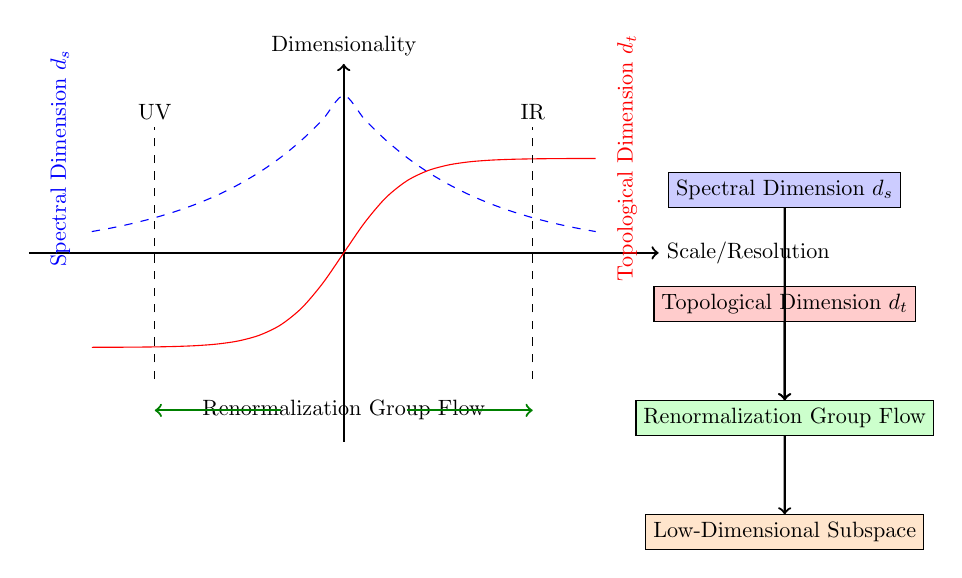
\begin{tikzpicture}[scale=0.8, every node/.style={scale=0.8}]
\draw[thick, ->] (-5,0) -- (5,0) node[right] {Scale/Resolution};
\draw[thick, ->] (0,-3) -- (0,3) node[above] {Dimensionality};

\draw[domain=-4:4,smooth,variable=\x,blue,dashed] plot ({\x},{2.5*exp(-abs(\x)/2)});
\node[blue,rotate=90] at (-4.5,1.5) {Spectral Dimension $d_s$};

\draw[domain=-4:4,smooth,variable=\x,red] plot ({\x},{1.5*tanh(\x)});
\node[red,rotate=90] at (4.5,1.5) {Topological Dimension $d_t$};

\draw[dashed] (-3,-2) -- (-3,2) node[above] {UV};
\draw[dashed] (3,-2) -- (3,2) node[above] {IR};

\node at (0,-2.5) {Renormalization Group Flow};
\draw[thick, ->, color=green!50!black] (-1,-2.5) -- (-3,-2.5);
\draw[thick, ->, color=green!50!black] (1,-2.5) -- (3,-2.5);

\begin{scope}[xshift=7cm, yshift=1cm, node distance=1cm]
\node[draw, rectangle, fill=blue!20] (SpectralDim) {Spectral Dimension $d_s$};
\node[draw, rectangle, fill=red!20, below=of SpectralDim] (TopologicalDim) {Topological Dimension $d_t$};
\node[draw, rectangle, fill=green!20, below=of TopologicalDim] (RGFlow) {Renormalization Group Flow};
\node[draw, rectangle, fill=orange!20, below=of RGFlow] (LowDim) {Low-Dimensional Subspace};
\draw[thick, ->] (SpectralDim) -- (RGFlow);
\draw[thick, ->] (TopologicalDim) -- (RGFlow);
\draw[thick, ->] (RGFlow) -- (LowDim);
\end{scope}
\end{tikzpicture}
\caption{Schematic representation of the dimensional reduction and the emergence of a low-dimensional subspace. The spectral dimension $d_s$ (blue dashed curve) measures the effective dimensionality of the space based on the return probability of a random walk, and it varies with the scale and resolution of the diffusion process. The topological dimension $d_t$ (red solid curve) measures the intrinsic dimensionality of the space based on its connectivity and topology, and it remains constant under the renormalization group flow (green arrows). The UV limit (left dashed line) corresponds to the high-energy and short-distance regime, where the spectral dimension is high and the space is highly connected and entangled. The IR limit (right dashed line) corresponds to the low-energy and long-distance regime, where the spectral dimension is low and the space is effectively low-dimensional and pseudo-rectilinear. The legend on the right explains the relationship between the spectral and topological dimensions, the renormalization group flow, and the emergence of a low-dimensional subspace.}
\label{fig:dimensional_reduction}
\end{figure}

\subsection{Fermionic fields and the emergence of matter particles}
The fermionic fields, such as the electron field, the quark fields, and the neutrino fields, also emerge from the connectivity graph of the emergent space, which describes the fermions as the excitations and fluctuations of the graph. The fermionic fields are characterized by the spinor representations of the Lorentz group, which describe the transformation properties of the fermions under the rotations and boosts of the emergent space. The fermionic fields are also characterized by the chiral symmetry, which describes the invariance of the fields under the transformations of the left-handed and right-handed components of the fermions.

\begin{tcolorbox}[colback=green!5!white,colframe=green!75!black,title=Question]
How does the emergence of the fundamental quantum fields from the connectivity graph relate to the idea of "it from bit" and the information-theoretic origin of the laws of physics?
\tcblower
The emergence of the fundamental quantum fields from the connectivity graph is closely related to the idea of "it from bit", which was proposed by John Wheeler as a way to understand the origin of the laws of physics from the fundamental principles of information theory. According to this idea, the physical reality is not made of matter or energy, but of information, and the laws of physics are the algorithms that process and transform this information.

In the context of our framework, the connectivity graph of the emergent space can be seen as a network of information, where each node represents a quantum state, and each edge represents a correlation or an interaction between the states. The quantum fields emerge as the collective excitations and the statistical properties of this network, which are determined by the topology and the geometry of the graph, and by the rules and the constraints that govern the dynamics and the evolution of the information.

The bosonic fields, such as the electromagnetic field or the gravitational field, can be interpreted as the carriers of the information, which mediate the interactions and the correlations between the states, and which give rise to the forces and the symmetries of the emergent space. The fermionic fields, such as the electron field or the quark fields, can be interpreted as the processors of the information, which encode and manipulate the quantum states, and which give rise to the matter and the structure of the emergent space.

The laws of physics, such as the equations of motion of the fields or the conservation laws of the charges and the currents, can be seen as the algorithms that describe the flow and the transformation of the information in the network, and that ensure the consistency and the stability of the emergent space. The gauge symmetries and the Lorentz symmetry of the fields can be seen as the redundancies and the invariances of the information, which reflect the underlying structure and the symmetries of the graph, and which allow to compress and to simplify the description of the emergent space.

The chiral symmetry of the fermionic fields can be seen as a signature of the handedness and the orientation of the information, which distinguishes between the left-handed and the right-handed components of the fermions, and which may be related to the arrow of time and the violation of the CP symmetry in the early universe.

Thus, the emergence of the fundamental quantum fields from the connectivity graph provides a concrete realization of the idea of "it from bit", and it offers a new perspective on the information-theoretic origin of the laws of physics, and on the role of information in the structure and the dynamics of the emergent space. This perspective may also have important implications for the nature of consciousness and the mind-body problem, as it suggests that the mental states and the qualia of the observers may be the subjective experiences of the information processing in the network, and that the physical states and the observables of the fields may be the objective manifestations of this processing in the emergent space.
\end{tcolorbox}

\section{Symmetry breaking and the Higgs mechanism}
\subsection{Electroweak symmetry breaking and the emergence of massive gauge bosons}
The emergent quantum fields undergo a series of symmetry breaking phase transitions, which lead to the formation of the massive gauge bosons and the Higgs boson. The electroweak symmetry breaking is driven by the Higgs mechanism, which describes the spontaneous breaking of the $SU(2) \times U(1)$ gauge symmetry of the electroweak field, and the emergence of the massive $W$ and $Z$ bosons, and the massless photon. The Higgs mechanism is based on the existence of a scalar field, called the Higgs field, which has a non-zero vacuum expectation value, and which couples to the gauge bosons and the fermions, giving them their masses.

\begin{tcolorbox}[colback=blue!5!white,colframe=blue!75!black,title=New terms]
\begin{description}
\item[Higgs mechanism:] A mechanism that explains the origin of the masses of the elementary particles in the standard model, and that provides a consistent way to break the gauge symmetries of the fields without violating the renormalizability and the unitarity of the theory. The Higgs mechanism is based on the existence of a scalar field, called the Higgs field, which has a non-zero vacuum expectation value, and which couples to the gauge bosons and the fermions, giving them their masses through the spontaneous symmetry breaking of the gauge symmetries.
\item[Electroweak symmetry:] The gauge symmetry of the electroweak field, which is a unified description of the electromagnetic and the weak interactions, and which is based on the $SU(2) \times U(1)$ group. The electroweak symmetry is spontaneously broken by the Higgs mechanism, which gives rise to the massive $W$ and $Z$ bosons, which mediate the weak interactions, and the massless photon, which mediates the electromagnetic interactions.
\end{description}
\end{tcolorbox}

\subsection{Chiral symmetry breaking and the emergence of massive fermions}
The chiral symmetry of the fermionic fields is also broken by the Higgs mechanism, which leads to the emergence of the massive fermions, such as the electrons, the quarks, and the neutrinos. The chiral symmetry breaking is driven by the Yukawa couplings between the Higgs field and the fermionic fields, which generate the mass terms for the fermions, and which mix the left-handed and right-handed components of the fermions. The chiral symmetry breaking is also related to the existence of the strong CP problem, which is the question of why the strong interaction does not violate the CP symmetry, and which is solved by the existence of the axion field.


\begin{figure}[h]
\centering
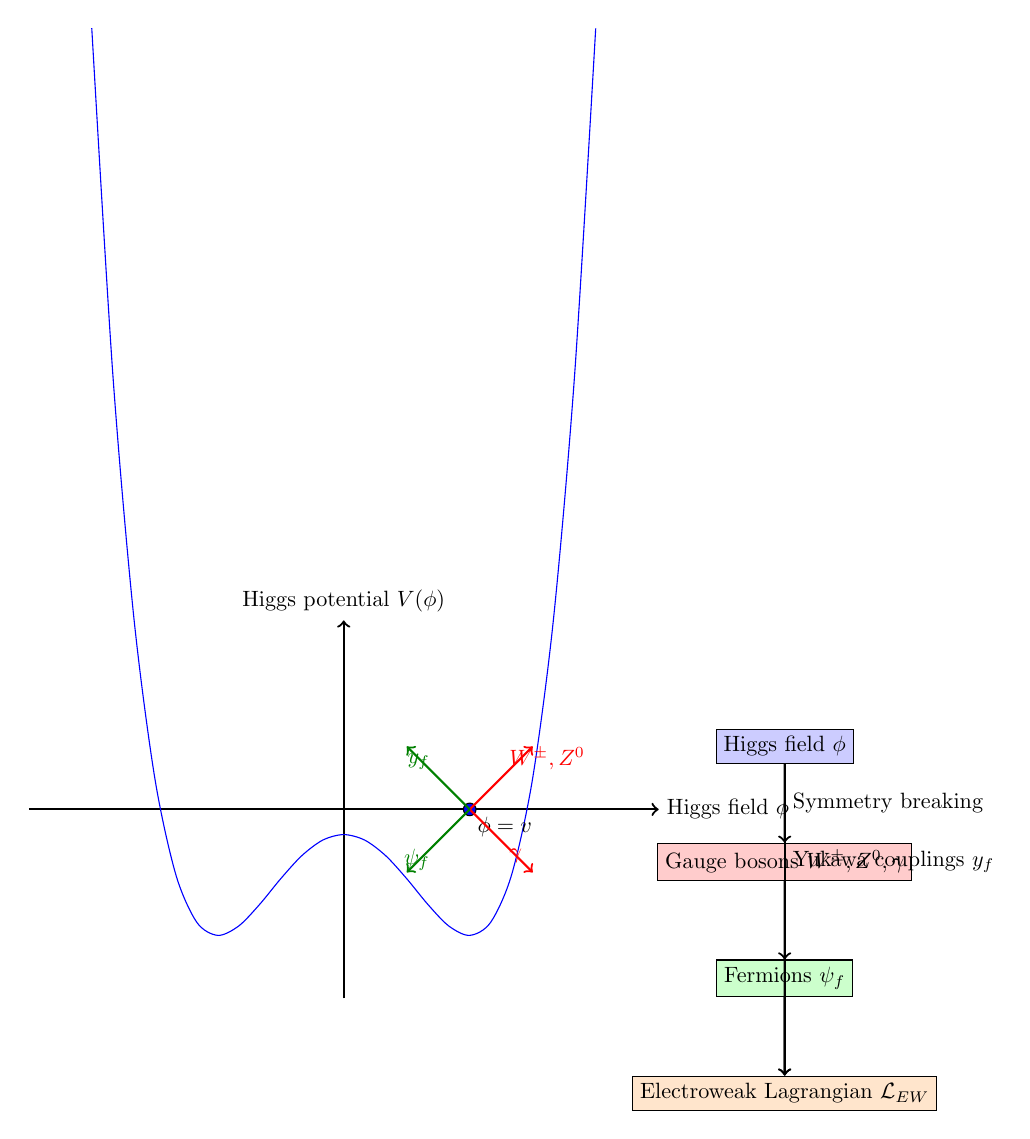
\begin{tikzpicture}[scale=0.8, every node/.style={scale=0.8}]
\draw[thick, ->] (-5,0) -- (5,0) node[right] {Higgs field $\phi$};
\draw[thick, ->] (0,-3) -- (0,3) node[above] {Higgs potential $V(\phi)$};

\draw[domain=-4:4,smooth,variable=\x,blue] plot ({\x},{0.1*(\x*\x-4)^2-2});
\draw[fill=blue] (2,0) circle (0.1) node[below right] {$\phi = v$};

\draw[thick, ->, color=red] (2,0) -- (3,1) node[midway,above right] {$W^{\pm}, Z^0$};
\draw[thick, ->, color=red] (2,0) -- (3,-1) node[midway,below right] {$\gamma$};

\draw[thick, ->, color=green!50!black] (2,0) -- (1,1) node[midway,above left] {$y_f$};
\draw[thick, ->, color=green!50!black] (2,0) -- (1,-1) node[midway,below left] {$\psi_f$};

\begin{scope}[xshift=7cm, yshift=1cm, node distance=1cm]
\node[draw, rectangle, fill=blue!20] (HiggsField) {Higgs field $\phi$};
\node[draw, rectangle, fill=red!20, below=of HiggsField] (GaugeBosons) {Gauge bosons $W^{\pm}, Z^0, \gamma$};
\node[draw, rectangle, fill=green!20, below=of GaugeBosons] (Fermions) {Fermions $\psi_f$};
\node[draw, rectangle, fill=orange!20, below=of Fermions] (Lagrangian) {Electroweak Lagrangian $\mathcal{L}_{EW}$};
\draw[thick, ->] (HiggsField) -- (GaugeBosons) node[midway, right] {Symmetry breaking};
\draw[thick, ->] (HiggsField) -- (Fermions) node[midway, right] {Yukawa couplings $y_f$};
\draw[thick, ->] (GaugeBosons) -- (Lagrangian);
\draw[thick, ->] (Fermions) -- (Lagrangian);
\end{scope}
\end{tikzpicture}
\caption{Schematic representation of the Higgs mechanism and the electroweak symmetry breaking. The Higgs field $\phi$ (blue curve) has a non-zero vacuum expectation value $v$ (blue dot), which breaks the $SU(2) \times U(1)$ gauge symmetry of the electroweak field, and which gives rise to the massive $W$ and $Z$ bosons, and the massless photon (red arrows). The Higgs field also couples to the fermionic fields $\psi_f$ through the Yukawa couplings $y_f$ (green arrows), which generate the mass terms for the fermions, and which break the chiral symmetry of the fields. The interactions between the Higgs field, the gauge bosons, and the fermions are described by the electroweak Lagrangian $\mathcal{L}_{EW}$ (orange box). The legend on the right explains the relationship between the Higgs mechanism, the electroweak symmetry breaking, the generation of particle masses, and the electroweak Lagrangian.}
\label{fig:higgs_mechanism}
\end{figure}

\begin{tcolorbox}[colback=green!5!white,colframe=green!75!black,title=Question]
What is the physical meaning and the origin of the Higgs field? Is it a fundamental field or an effective description of some deeper structure?
\tcblower
The physical meaning and the origin of the Higgs field is one of the most important questions in modern particle physics, and it is still a subject of active research and debate. In the standard model, the Higgs field is introduced as a fundamental scalar field, which has a non-zero vacuum expectation value, and which is responsible for the generation of the masses of the elementary particles through the Higgs mechanism. However, the standard model does not provide an explanation for the origin and the nature of the Higgs field, or for the specific form of its potential and its couplings to the other fields.

In the context of our framework, the Higgs field can be seen as an effective description of the collective behavior and the symmetry breaking of the underlying degrees of freedom of the USMS, which are represented by the connectivity graph of the emergent space. The Higgs field emerges as a coarse-grained and averaged description of the fluctuations and the correlations of the graph, which are induced by the morphic resonance and the self-organization of the states, and which break the symmetries of the graph and give rise to the structured and stable patterns of the emergent space.

The non-zero vacuum expectation value of the Higgs field can be interpreted as a measure of the coherence and the stability of the graph, which is maintained by the balance between the local interactions and the global constraints of the states, and which is resistant to the perturbations and the deformations of the graph. The potential of the Higgs field can be seen as a phenomenological description of the energy landscape and the phase diagram of the graph, which has a minimum at the vacuum expectation value, and which determines the possible configurations and the transitions of the graph.

The couplings of the Higgs field to the gauge bosons and the fermions can be seen as a reflection of the topological and the geometric properties of the graph, which are encoded in the connectivity and the curvature of the graph, and which give rise to the interactions and the symmetries of the emergent fields. The gauge bosons can be seen as the topological excitations of the graph, which are associated with the cycles and the holes of the graph, and which mediate the long-range correlations and the forces between the states. The fermions can be seen as the geometric excitations of the graph, which are associated with the nodes and the links of the graph, and which represent the localized and the propagating degrees of freedom of the emergent space.

In this perspective, the Higgs field is not a fundamental field, but an effective description of the collective behavior and the symmetry breaking of the underlying degrees of freedom of the USMS, which are represented by the connectivity graph of the emergent space. The Higgs field is an emergent phenomenon, which arises from the self-organization and the phase transitions of the graph, and which reflects the topological and the geometric properties of the graph, and the interactions and the symmetries of the emergent fields.

This interpretation of the Higgs field is consistent with the idea of the "it from bit" and the information-theoretic origin of the laws of physics, as it suggests that the Higgs field is a manifestation of the information processing and the computation of the graph, which gives rise to the structure and the dynamics of the emergent space, and which encodes the fundamental principles and the algorithms of the universe. It is also consistent with the idea of the "emergence of spacetime" and the "quantum gravity", as it suggests that the Higgs field is a bridge between the quantum and the classical descriptions of the emergent space, and that it plays a crucial role in the transition from the pre-geometric and the non-spatial phases of the USMS to the geometric and the spatial phases of the emergent space.
\end{tcolorbox}

\section{Renormalization group flow and the scale-dependent behavior of quantum fields}
\subsection{Asymptotic freedom and the ultraviolet limit}
The behavior of the quantum fields at high energies and short distances is described by the renormalization group flow, which is the process of changing the scale and the resolution of the fields, and which leads to the emergence of the effective field theories. The renormalization group flow of the strong interaction is characterized by the property of asymptotic freedom, which means that the coupling constant of the strong interaction decreases at high energies and short distances, and which leads to the confinement of the quarks and the gluons at low energies and long distances. The ultraviolet limit of the renormalization group flow corresponds to the high-energy and short-distance limit of the fields, which is characterized by the existence of the Landau poles, and which requires the existence of a fundamental theory that describes the fields at the Planck scale.

\begin{tcolorbox}[colback=blue!5!white,colframe=blue!75!black,title=New terms]
\begin{description}
\item[Renormalization group:] A mathematical framework that describes the change of the parameters and the couplings of a physical theory as a function of the energy scale or the length scale of the observations. The renormalization group is based on the idea of the scale invariance and the self-similarity of the physical systems, and it allows to study the behavior of the systems at different scales, and to identify the relevant and the irrelevant degrees of freedom at each scale.
\item[Asymptotic freedom:] A property of the strong interaction, which means that the coupling constant of the interaction decreases at high energies and short distances, and which leads to the confinement of the quarks and the gluons at low energies and long distances. Asymptotic freedom is a consequence of the non-Abelian nature of the strong interaction, and it is one of the key features of the quantum chromodynamics, which is the theory of the strong interaction in the standard model.
\end{description}
\end{tcolorbox}

\subsection{Infrared fixed points and the emergence of effective field theories}
The behavior of the quantum fields at low energies and long distances is described by the effective field theories, which are the approximate and simplified descriptions of the fields, that capture the relevant degrees of freedom and the symmetries of the system. The effective field theories are characterized by the existence of the infrared fixed points, which are the scale-invariant and self-similar configurations of the fields, that are stable under the renormalization group flow. The infrared fixed points of the renormalization group flow correspond to the low-energy and long-distance limit of the fields, which is characterized by the emergence of the classical and macroscopic behavior of the fields, and which is described by the equations of classical field theory and hydrodynamics.


\begin{figure}[h]
\centering
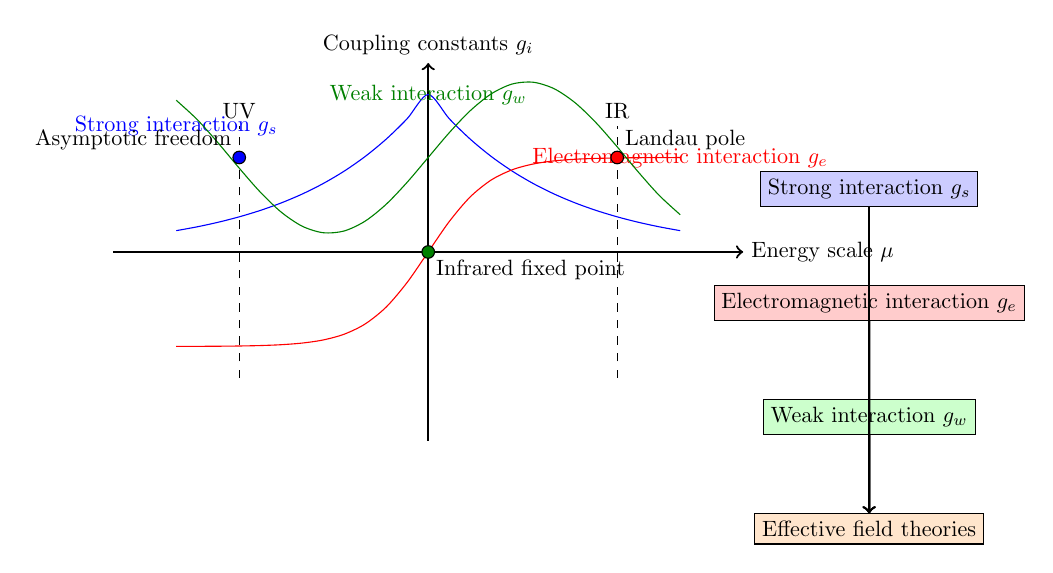
\begin{tikzpicture}[scale=0.8, every node/.style={scale=0.8}]
\draw[thick, ->] (-5,0) -- (5,0) node[right] {Energy scale $\mu$};
\draw[thick, ->] (0,-3) -- (0,3) node[above] {Coupling constants $g_i$};

\draw[domain=-4:4,smooth,variable=\x,blue] plot ({\x},{2.5*exp(-abs(\x)/2)});
\node[blue] at (-4,2) {Strong interaction $g_s$};

\draw[domain=-4:4,smooth,variable=\x,red] plot ({\x},{1.5*tanh(\x)});
\node[red] at (4,1.5) {Electromagnetic interaction $g_e$};

\draw[domain=-4:4,smooth,variable=\x,green!50!black] plot ({\x},{1.2*sin(deg(\x))+1.5});
\node[green!50!black] at (0,2.5) {Weak interaction $g_w$};

\draw[dashed] (-3,-2) -- (-3,2) node[above] {UV};
\draw[dashed] (3,-2) -- (3,2) node[above] {IR};

\draw[fill=blue] (-3,1.5) circle (0.1) node[above left] {Asymptotic freedom};
\draw[fill=red] (3,1.5) circle (0.1) node[above right] {Landau pole};
\draw[fill=green!50!black] (0,0) circle (0.1) node[below right] {Infrared fixed point};

\begin{scope}[xshift=7cm, yshift=1cm, node distance=1cm]
\node[draw, rectangle, fill=blue!20] (StrongInt) {Strong interaction $g_s$};
\node[draw, rectangle, fill=red!20, below=of StrongInt] (EMInt) {Electromagnetic interaction $g_e$};
\node[draw, rectangle, fill=green!20, below=of EMInt] (WeakInt) {Weak interaction $g_w$};
\node[draw, rectangle, fill=orange!20, below=of WeakInt] (EffectiveTheories) {Effective field theories};
\draw[thick, ->] (StrongInt) -- (EffectiveTheories);
\draw[thick, ->] (EMInt) -- (EffectiveTheories);
\draw[thick, ->] (WeakInt) -- (EffectiveTheories);
\end{scope}
\end{tikzpicture}
\caption{Schematic representation of the renormalization group flow and the scale-dependent behavior of the quantum fields. The figure shows the evolution of the coupling constants $g_i$ of the strong (blue curve), electromagnetic (red curve), and weak (green curve) interactions as a function of the energy scale $\mu$, from the ultraviolet (UV) to the infrared (IR) limit. The UV limit (left dashed line) is characterized by the asymptotic freedom of the strong interaction (blue dot), which leads to the decrease of the coupling constant $g_s$ at high energies, and by the Landau poles of the other interactions (red dot), which signal the breakdown of the perturbative description of the fields. The IR limit (right dashed line) is characterized by the emergence of the effective field theories (orange box), which are described by the infrared fixed points $g_i^*$ of the renormalization group flow (green dot), and which capture the relevant degrees of freedom and the symmetries of the system at low energies. The figure also shows the possible phase transitions and the symmetry breaking patterns of the fields, which are indicated by the bifurcations and the discontinuities of the flow lines. The legend on the right explains the relationship between the different interactions, the renormalization group flow, and the emergence of effective field theories.}
\label{fig:renormalization_group}
\end{figure}

%----------------------------------------------------------------------------------------
\newpage
\chapter{The Emergence of Gravity and Spacetime}\label{ch:TheEmergenceofGravityandSpacetime}

\section{Emergence of gravity from the curvature of the connectivity graph}
\subsection{Ricci curvature and the emergence of the metric tensor}
The emergent 3D space is not a flat and static background, but a dynamical and curved manifold, that is described by the metric tensor, which encodes the distances and angles between the points of the space. The metric tensor emerges from the curvature of the connectivity graph of the emergent space, which is described by the Ricci curvature, that measures the deviation of the graph from a flat and regular lattice. The Ricci curvature is a local and intrinsic property of the graph, that depends on the connectivity and the topology of the graph, and that determines the geodesics and the parallel transport of the vectors on the graph.

\begin{tcolorbox}[colback=blue!5!white,colframe=blue!75!black,title=New terms]
\begin{description}
\item[Metric tensor:] A symmetric and non-degenerate tensor field $g_{\mu\nu}$, that defines the geometry and the curvature of a manifold, and that encodes the distances and the angles between the points of the manifold. The metric tensor is the fundamental object of the general relativity, and it satisfies the Einstein field equations, which relate the curvature of the spacetime to the energy and the momentum of the matter fields.
\item[Ricci curvature:] A geometric quantity that measures the deviation of a manifold from a flat and homogeneous space, and that is defined as the contraction of the Riemann curvature tensor $R_{\mu\nu\rho\sigma}$ with respect to two of its indices. The Ricci curvature $R_{\mu\nu}$ is a symmetric tensor that describes the local and intrinsic curvature of the manifold, and that enters the Einstein field equations as the source term for the metric tensor.
\end{description}
\end{tcolorbox}

\subsection{Einstein-Hilbert action and the derivation of the Einstein field equations}
The dynamics of the emergent spacetime is described by the Einstein-Hilbert action, which is a functional of the metric tensor, that measures the curvature and the topology of the spacetime, and that determines the equations of motion of the metric tensor. The Einstein-Hilbert action is derived from the principle of least action, which states that the metric tensor evolves in such a way that minimizes the action, and which leads to the Einstein field equations, that relate the curvature of the spacetime to the energy and the momentum of the matter fields. The Einstein field equations are a set of non-linear and coupled partial differential equations, that describe the feedback between the curvature of the spacetime and the distribution of the matter fields, and that determine the large-scale structure and the evolution of the universe.

\begin{tcolorbox}[colback=green!5!white,colframe=green!75!black,title=Question]
How does the emergence of gravity from the curvature of the connectivity graph relate to the problem of quantum gravity and the unification of general relativity and quantum mechanics?
\tcblower
The emergence of gravity from the curvature of the connectivity graph provides a new perspective on the problem of quantum gravity and the unification of general relativity and quantum mechanics, which are two of the most fundamental and successful theories of modern physics, but which are also incompatible and inconsistent with each other at the Planck scale.

In general relativity, gravity is described as the curvature of the spacetime, which is a smooth and continuous manifold that obeys the Einstein field equations, and which is not affected by the quantum fluctuations and the discreteness of the matter fields. In quantum mechanics, the matter fields are described as the excitations and the superpositions of the quantum states, which obey the laws of quantum mechanics, such as the Heisenberg uncertainty principle and the Schrödinger equation, and which can have non-local and entangled correlations that are not possible in classical physics.

The incompatibility between general relativity and quantum mechanics arises from the fact that the spacetime is a dynamical and fluctuating entity in quantum gravity, which is subject to the same quantum laws and the same quantum fluctuations as the matter fields, and which cannot be described as a smooth and continuous manifold at the Planck scale. This leads to the problem of the non-renormalizability of the perturbative quantum gravity, which means that the theory is not well-defined and predictive at high energies, and to the problem of the singularities and the information loss in black holes, which violate the unitarity and the conservation of probabilities in quantum mechanics.

In the context of our framework, the emergence of gravity from the curvature of the connectivity graph offers a possible solution to these problems, by providing a non-perturbative and background-independent formulation of quantum gravity, which is based on the fundamental degrees of freedom and the symmetries of the USMS, and which does not rely on the assumption of a fixed and classical spacetime. In this formulation, the spacetime is not a fundamental entity, but an emergent phenomenon that arises from the collective behavior and the phase transitions of the underlying degrees of freedom, which are described by the connectivity graph of the emergent space.

The curvature of the connectivity graph, which is described by the Ricci curvature, is not a classical and deterministic quantity, but a quantum and fluctuating property that reflects the entanglement and the correlations of the states in the graph, and that obeys the laws of quantum mechanics, such as the superposition principle and the uncertainty principle. The metric tensor, which encodes the geometry and the curvature of the emergent spacetime, is not a fundamental field, but an effective description of the collective behavior and the symmetry breaking of the graph, which is derived from the Einstein-Hilbert action, and which satisfies the Einstein field equations in the classical limit.

In this perspective, the problem of quantum gravity is not the problem of quantizing the classical spacetime, or of finding a consistent theory that describes the quantum fluctuations of the metric tensor, but the problem of understanding the emergence of the classical spacetime from the fundamental degrees of freedom and the symmetries of the USMS, and of deriving the Einstein field equations and the other laws of gravity from the principles of quantum mechanics and the properties of the connectivity graph.

This approach to quantum gravity is similar to the idea of the "emergent gravity" and the "entropic gravity", which have been proposed by various authors as a way to reconcile general relativity and quantum mechanics, and to explain the origin of gravity as an entropic force that arises from the statistical properties and the information content of the underlying degrees of freedom. However, our framework differs from these approaches in several key aspects, such as the nature and the properties of the fundamental degrees of freedom, the role of the morphic resonance and the self-organization in the emergence of the spacetime, and the relation between the quantum and the classical descriptions of the emergent gravity.

In our framework, the fundamental degrees of freedom are not the quantum bits or the holographic screens, but the states and the correlations of the USMS, which are described by the connectivity graph of the emergent space, and which have a complex and hierarchical structure that reflects the non-local and non-linear nature of the morphic resonance and the self-organization. The emergence of the spacetime is not a purely entropic or thermodynamic process, but a quantum and dynamical process that involves the symmetry breaking and the phase transitions of the graph, and that is driven by the competition and the cooperation between the local interactions and the global constraints of the states.

The relation between the quantum and the classical descriptions of the emergent gravity is not a simple correspondence or a duality, but a complex and multi-scale process that involves the renormalization and the coarse-graining of the graph, and that leads to the emergence of the effective field theories and the classical equations of motion in the infrared limit. The quantum fluctuations and the discreteness of the graph are not negligible or irrelevant at the Planck scale, but they are the essential and the dominant features of the emergent gravity, which determine the structure and the dynamics of the spacetime at the fundamental level, and which require a non-perturbative and background-independent formulation of quantum gravity.

In summary, the emergence of gravity from the curvature of the connectivity graph provides a new and promising approach to the problem of quantum gravity and the unification of general relativity and quantum mechanics, which is based on the fundamental degrees of freedom and the symmetries of the USMS, and which offers a non-perturbative and background-independent formulation of quantum gravity that is consistent with the principles of quantum mechanics and the properties of the emergent spacetime. This approach opens new avenues for the exploration and the understanding of the nature of gravity and the origin of the universe, and it has important implications for the foundations of physics and the philosophy of science.
\end{tcolorbox}

\section{Relationship between gravity, quantum fields, and the structure of 3D space}
\subsection{Quantum gravity and the unification of general relativity and quantum field theory}
The emergence of gravity from the curvature of the connectivity graph is a manifestation of the deep connection between gravity, quantum fields, and the structure of 3D space. The unification of general relativity and quantum field theory requires the formulation of a theory of quantum gravity, that describes the quantum properties and the fluctuations of the spacetime, and that resolves the singularities and the inconsistencies of the classical theory. The theory of quantum gravity is based on the idea that the spacetime is a quantum object, that is described by a quantum state, and that obeys the laws of quantum mechanics, such as the superposition principle and the uncertainty principle.

\begin{tcolorbox}[colback=blue!5!white,colframe=blue!75!black,title=New terms]
\begin{description}
\item[Quantum gravity:] A theory that describes the quantum properties and the fluctuations of the spacetime, and that unifies the principles of general relativity and quantum mechanics. Quantum gravity is necessary to resolve the singularities and the inconsistencies of the classical theory of gravity, such as the black hole singularities and the initial singularity of the Big Bang, and to provide a consistent description of the spacetime at the Planck scale, where the quantum effects become dominant.
\item[Superposition principle:] A fundamental principle of quantum mechanics, which states that a quantum system can exist in a superposition of multiple states, and that the probability of measuring a particular state is given by the square of the absolute value of the amplitude of that state in the superposition. The superposition principle is a consequence of the linearity of the Schrödinger equation, and it leads to the phenomenon of quantum interference and entanglement.
\end{description}
\end{tcolorbox}

\subsection{Holographic principle and the emergence of spacetime from quantum entanglement}
The holographic principle states that the information and the degrees of freedom of a region of spacetime are encoded on the boundary of the region, and that the boundary theory is a quantum field theory that lives in one less dimension than the bulk theory. The holographic principle implies that the emergent spacetime is a hologram, that is projected from the quantum entanglement and the correlations of the boundary theory, and that the geometry and the topology of the spacetime are emergent properties of the entanglement structure of the boundary theory. The emergence of spacetime from quantum entanglement is a manifestation of the deep connection between gravity, quantum information, and the structure of 3D space, and it suggests that the spacetime is a quantum error-correcting code, that protects the information and the coherence of the boundary theory from the errors and the decoherence of the bulk theory.


\begin{figure}[h]
\centering
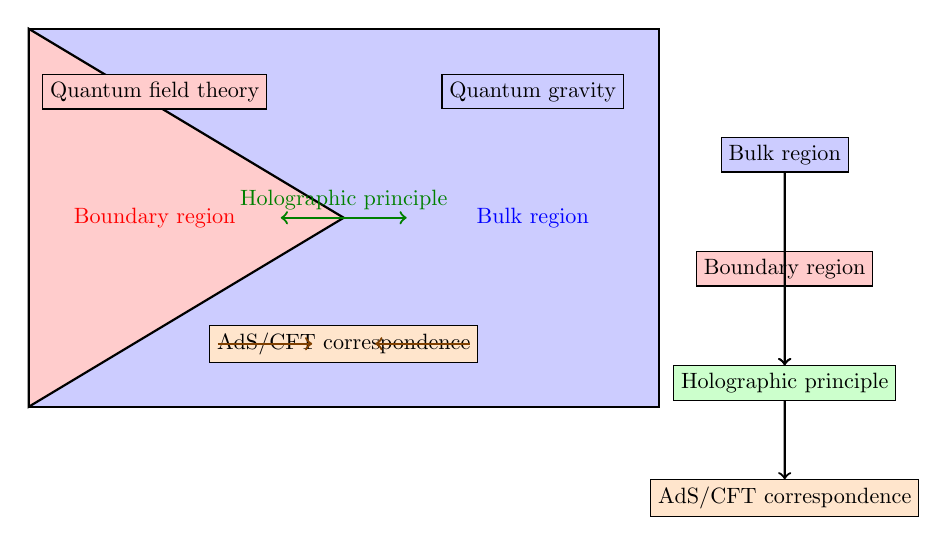
\begin{tikzpicture}[scale=0.8, every node/.style={scale=0.8}]
\draw[thick, fill=blue!20] (-5,-3) -- (-5,3) -- (5,3) -- (5,-3) -- cycle;
\draw[thick, fill=red!20] (-5,-3) -- (-5,3) -- (0,0) -- cycle;

\node[blue] at (3,0) {Bulk region};
\node[red] at (-3,0) {Boundary region};

\node[draw, rectangle, fill=blue!20] at (3,2) {Quantum gravity};
\node[draw, rectangle, fill=red!20] at (-3,2) {Quantum field theory};

\draw[thick, <->, color=green!50!black] (-1,0) -- (1,0) node[midway,above] {Holographic principle};

\node[draw, rectangle, fill=orange!20] at (0,-2) {AdS/CFT correspondence};
\draw[thick, ->, color=orange!50!black] (-2,-2) -- (-0.5,-2);
\draw[thick, ->, color=orange!50!black] (2,-2) -- (0.5,-2);

\begin{scope}[xshift=7cm, yshift=1cm, node distance=1cm]
\node[draw, rectangle, fill=blue!20] (BulkRegion) {Bulk region};
\node[draw, rectangle, fill=red!20, below=of BulkRegion] (BoundaryRegion) {Boundary region};
\node[draw, rectangle, fill=green!20, below=of BoundaryRegion] (HolographicPrinciple) {Holographic principle};
\node[draw, rectangle, fill=orange!20, below=of HolographicPrinciple] (AdSCFT) {AdS/CFT correspondence};
\draw[thick, ->] (BulkRegion) -- (HolographicPrinciple);
\draw[thick, ->] (BoundaryRegion) -- (HolographicPrinciple);
\draw[thick, ->] (HolographicPrinciple) -- (AdSCFT);
\end{scope}
\end{tikzpicture}
\caption{Schematic representation of the holographic principle and the emergence of spacetime from quantum entanglement. The figure shows a region of spacetime, which is divided into a bulk region (blue) and a boundary region (red). The bulk region is described by a theory of quantum gravity (blue box), such as string theory or loop quantum gravity, which describes the quantum fluctuations and the discreteness of the spacetime. The boundary region is described by a quantum field theory (red box), such as a conformal field theory or a matrix model, which lives in one less dimension than the bulk theory, and which encodes the information and the degrees of freedom of the bulk region. The geometry and the topology of the bulk spacetime emerge from the entanglement structure and the correlations of the boundary theory, which are described by the tensor network and the holographic entanglement entropy (green arrow). The figure also shows the AdS/CFT correspondence (orange box and arrows), which is a concrete realization of the holographic principle, and which relates a theory of gravity in an anti-de Sitter (AdS) space to a conformal field theory (CFT) on the boundary of the AdS space. The legend on the right explains the relationship between the bulk and boundary regions, the holographic principle, and the AdS/CFT correspondence.}
\label{fig:holographic_principle}
\end{figure}

\begin{tcolorbox}[colback=green!5!white,colframe=green!75!black,title=Question]
What is the physical meaning and the implications of the holographic principle for the nature of space and time? Is the holographic principle a fundamental principle of nature or an emergent property of quantum gravity?
\tcblower
The physical meaning and the implications of the holographic principle for the nature of space and time are profound and far-reaching, and they challenge some of the most basic assumptions and intuitions about the structure and the dimensionality of the universe.

At the most fundamental level, the holographic principle implies that the spacetime is not a fundamental entity, but an emergent phenomenon that arises from the quantum entanglement and the correlations of the underlying degrees of freedom, which live in a lower-dimensional boundary theory. This means that the three spatial dimensions and the one temporal dimension of the observable universe are not intrinsic properties of the spacetime, but are the result of the projection and the encoding of the information and the degrees of freedom of the boundary theory, which may have a different dimensionality and a different geometry than the bulk spacetime.

The holographic principle also implies that the quantum gravity and the quantum field theory are not independent and separate theories, but are the two sides of the same coin, which are related by a duality and a correspondence that maps the properties and the observables of one theory to the other. This means that the quantum fluctuations and the discreteness of the spacetime, which are described by the theory of quantum gravity in the bulk, are equivalent and dual to the quantum entanglement and the correlations of the matter fields, which are described by the quantum field theory on the boundary.

The holographic principle has important implications for the nature of space and time, and for the structure and the evolution of the universe. It suggests that the spacetime is not a passive and static background, but a dynamic and active participant in the quantum processes and the information flows of the universe, which can be created, destroyed, and transformed by the interactions and the measurements of the observers and the measuring devices. It also suggests that the spacetime is not a continuous and smooth manifold, but a discrete and fluctuating network of quantum bits and quantum gates, which are constantly being updated and processed by the quantum computations and the quantum error-corrections of the boundary theory.

The holographic principle also has important implications for the problem of quantum gravity and the unification of general relativity and quantum mechanics. It provides a new perspective and a new approach to the problem of quantizing gravity and spacetime, which is based on the idea of emergent spacetime and holographic duality, and which avoids some of the difficulties and the inconsistencies of the conventional approaches, such as string theory and loop quantum gravity. It also offers a new framework and a new language for the formulation of a theory of quantum gravity, which is based on the principles of quantum information and quantum computation, and which may lead to new insights and new predictions about the nature of space and time, and the origin and the fate of the universe.

However, the holographic principle is still a conjecture and a hypothesis, which has not been fully proven or tested experimentally, and which has some limitations and open questions that need to be addressed and resolved. One of the main questions is whether the holographic principle is a fundamental principle of nature, which holds for all the systems and all the scales of the universe, or an emergent property of quantum gravity, which is valid only in certain regimes and under certain conditions, such as the strong coupling limit or the large N limit of the boundary theory.

Another question is how to generalize and extend the holographic principle to the case of dynamical and time-dependent spacetimes, which are not asymptotically anti-de Sitter or flat, and which may have singularities or horizons that affect the structure and the evolution of the boundary theory. A related question is how to incorporate the effects of matter and energy on the geometry and the topology of the spacetime, and how to derive the Einstein field equations and the other laws of gravity from the principles of the holographic principle and the properties of the boundary theory.

A third question is how to interpret and explain the holographic principle in terms of the fundamental principles and the physical mechanisms of the universe, and how to relate it to the other principles and the other theories of physics, such as the second law of thermodynamics, the principle of least action, the gauge principle, and the standard model of particle physics. This requires a deeper understanding and a more general formulation of the holographic principle, which goes beyond the specific examples and the mathematical techniques of the AdS/CFT correspondence and the other holographic dualities, and which provides a unified and consistent picture of the nature of space and time, and the origin and the structure of the universe.

In conclusion, the holographic principle is a profound and revolutionary idea that challenges our understanding of the nature of space and time, and that opens new horizons and new directions for the exploration and the explanation of the fundamental laws and the ultimate constituents of the universe. Whether it is a fundamental principle of nature or an emergent property of quantum gravity, the holographic principle has important implications and consequences for the foundations of physics and the philosophy of science, and it requires a careful and critical examination and a creative and imaginative approach to the problem of quantum gravity and the unification of general relativity and quantum mechanics.
\end{tcolorbox}

\section{Cosmological implications and the evolution of the universe}
\subsection{Big Bang singularity and the initial conditions of the universe}
The emergence of spacetime from the connectivity graph has important implications for the cosmology and the evolution of the universe, and it provides a new perspective on the origin and the initial conditions of the universe. The Big Bang singularity, which is the initial state of the universe in the standard cosmological model, is replaced by a quantum state of the connectivity graph, that describes the entanglement and the correlations of the degrees of freedom of the graph, and that determines the initial conditions and the symmetries of the emergent spacetime. The quantum state of the connectivity graph is described by a wave function, that obeys the Wheeler-DeWitt equation, which is the quantum version of the Einstein-Hilbert equation, and that describes the evolution and the fluctuations of the wave function in the space of geometries and topologies.

\begin{tcolorbox}[colback=blue!5!white,colframe=blue!75!black,title=New terms]
\begin{description}
\item[Big Bang singularity:] The initial state of the universe in the standard cosmological model, which is characterized by an infinite density and temperature, and a vanishing volume and radius of the spacetime. The Big Bang singularity is a consequence of the extrapolation of the classical equations of general relativity to the extreme conditions of the early universe, and it represents a breakdown of the classical theory, which requires a quantum description of gravity and spacetime.
\item[Wheeler-DeWitt equation:] The quantum version of the Einstein-Hilbert equation, which describes the evolution and the fluctuations of the wave function of the universe in the space of geometries and topologies. The Wheeler-DeWitt equation is a functional differential equation, which is derived from the Hamiltonian formulation of general relativity, and which takes the form $\mathcal{H}\Psi[g] = 0$, where $\mathcal{H}$ is the Hamiltonian operator, $\Psi[g]$ is the wave function of the universe, and $g$ is the metric tensor of the spacetime.
\end{description}
\end{tcolorbox}

\subsection{Inflation and the emergence of classical spacetime}
The evolution of the universe from the quantum state of the connectivity graph to the classical spacetime is described by the process of inflation, which is a period of exponential expansion of the universe, that amplifies the quantum fluctuations of the graph, and that generates the large-scale structure and the homogeneity of the universe. The inflation is driven by a scalar field, called the inflaton, that has a slow-roll potential, and that dominates the energy density of the universe during the inflation, and that decays into the standard model particles and the dark matter after the inflation. The emergence of classical spacetime from the quantum state of the connectivity graph is a consequence of the decoherence and the entanglement of the degrees of freedom of the graph, that leads to the formation of a classical background spacetime, and that suppresses the quantum fluctuations and the interferences of the graph.

\begin{figure}[h]
\centering
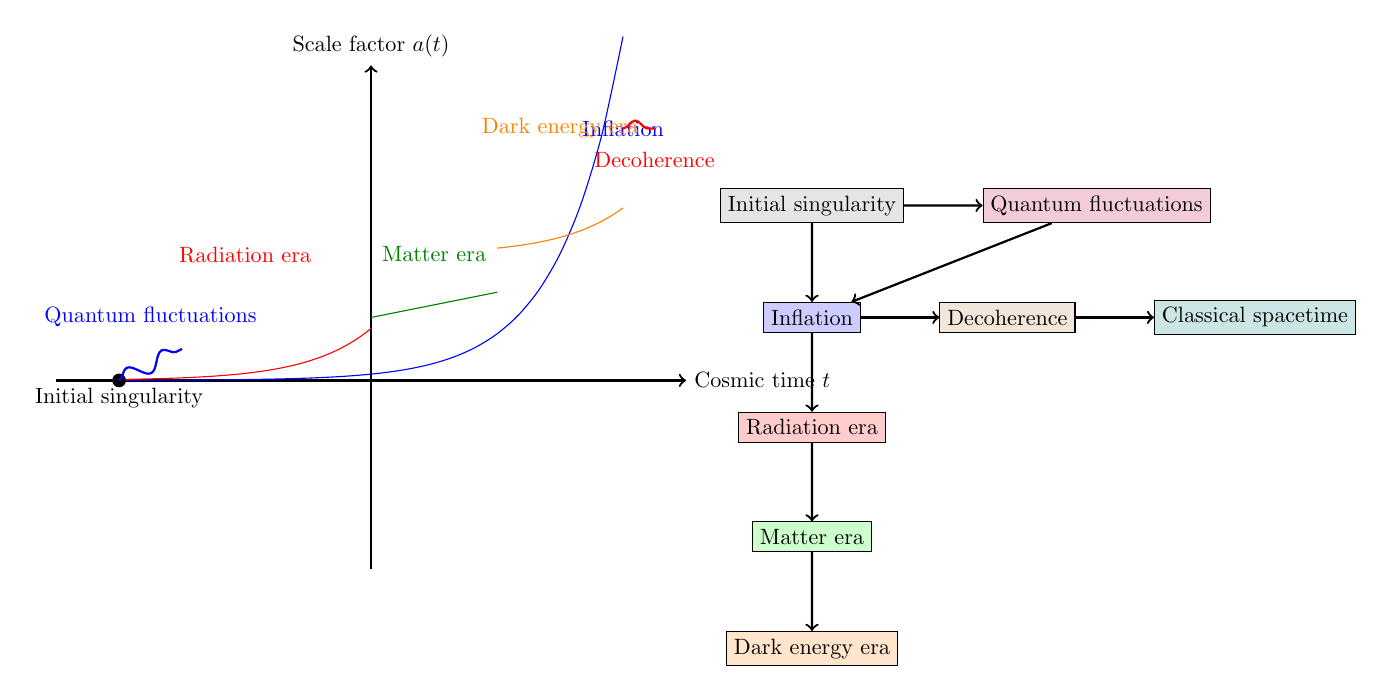
\begin{tikzpicture}[scale=0.8, every node/.style={scale=0.8}]
\draw[thick, ->] (-5,0) -- (5,0) node[right] {Cosmic time $t$};
\draw[thick, ->] (0,-3) -- (0,5) node[above] {Scale factor $a(t)$};

\draw[domain=-4:4,smooth,variable=\x,blue] plot ({\x},{0.1*exp(\x)});
\node[blue] at (4,4) {Inflation};

\draw[domain=-4:0,smooth,variable=\x,red] plot ({\x},{0.5*exp(0.5\x)});
\node[red] at (-2,2) {Radiation era};

\draw[domain=0:2,smooth,variable=\x,green!50!black] plot ({\x},{1+0.2*\x});
\node[green!50!black] at (1,2) {Matter era};

\draw[domain=2:4,smooth,variable=\x,orange] plot ({\x},{2+0.1*exp(\x-2)});
\node[orange] at (3,4) {Dark energy era};

\draw[fill=black] (-4,0) circle (0.1) node[below] {Initial singularity};

\draw[thick, color=blue, decorate, decoration={snake, amplitude=1mm, segment length=5mm}] (-4,0) -- (-3,0.5);
\node[blue] at (-3.5,1) {Quantum fluctuations};

\draw[thick, color=red, decorate, decoration={snake, amplitude=1mm, segment length=5mm}] (4,4) -- (4.5,4);
\node[red] at (4.5,3.5) {Decoherence};

\begin{scope}[xshift=7cm, yshift=1cm, node distance=1cm]
\node[draw, rectangle, fill=blue!20] (InflationEra) {Inflation};
\node[draw, rectangle, fill=red!20, below=of InflationEra] (RadiationEra) {Radiation era};
\node[draw, rectangle, fill=green!20, below=of RadiationEra] (MatterEra) {Matter era};
\node[draw, rectangle, fill=orange!20, below=of MatterEra] (DarkEnergyEra) {Dark energy era};
\node[draw, rectangle, fill=gray!20, above=of InflationEra] (InitialSingularity) {Initial singularity};
\node[draw, rectangle, fill=purple!20, right=of InitialSingularity] (QuantumFluctuations) {Quantum fluctuations};
\node[draw, rectangle, fill=brown!20, right=of InflationEra] (Decoherence) {Decoherence};
\node[draw, rectangle, fill=teal!20, right=of Decoherence] (ClassicalSpacetime) {Classical spacetime};
\draw[thick, ->] (InitialSingularity) -- (InflationEra);
\draw[thick, ->] (InflationEra) -- (RadiationEra);
\draw[thick, ->] (RadiationEra) -- (MatterEra);
\draw[thick, ->] (MatterEra) -- (DarkEnergyEra);
\draw[thick, ->] (InitialSingularity) -- (QuantumFluctuations);
\draw[thick, ->] (QuantumFluctuations) -- (InflationEra);
\draw[thick, ->] (InflationEra) -- (Decoherence);
\draw[thick, ->] (Decoherence) -- (ClassicalSpacetime);
\end{scope}
\end{tikzpicture}
\caption{Schematic representation of the inflation and the emergence of classical spacetime from the quantum state of the connectivity graph. The figure shows the evolution of the scale factor $a(t)$ of the universe as a function of the cosmic time $t$, from the initial singularity (black dot) to the present epoch. The initial singularity is replaced by a quantum state of the connectivity graph, which is described by a wave function $\Psi[g]$ that obeys the Wheeler-DeWitt equation. The wave function evolves and fluctuates in the space of geometries and topologies (blue wavy line), and it generates the initial conditions and the symmetries of the emergent spacetime. The inflation (blue curve) is a period of exponential expansion of the universe, which is driven by the inflaton field $\phi(t)$, and which amplifies the quantum fluctuations of the graph, and generates the large-scale structure and the homogeneity of the universe. The inflation ends when the inflaton field decays into the standard model particles and the dark matter, and the universe enters the radiation-dominated era (red curve), followed by the matter-dominated era (green curve) and the dark energy-dominated era (orange curve). The emergence of classical spacetime is a consequence of the decoherence and the entanglement of the degrees of freedom of the graph (red wavy line), which leads to the formation of a classical background spacetime, and the suppression of the quantum fluctuations and the interferences of the graph. The legend on the right explains the relationship between the different eras and phases of the universe, the quantum fluctuations, the decoherence, and the emergence of classical spacetime.}
\label{fig:inflation}
\end{figure}
%----------------------------------------------------------------------------------------
\newpage
\chapter{Conclusion and Future Directions}\label{ch:ConclusionandFutureDirections}

\section{Summary of the main results and insights}
\subsection{Emergence of 3D space from undifferentiated symmetric morphological space}
In this thesis, we have presented a novel framework for understanding the emergence of 3D space from an undifferentiated symmetric morphological space, using the tools of graph theory, quantum measurement theory, and morphic resonance. We have shown that the emergence of 3D space is a result of the interplay between the measurement-induced symmetry breaking and the morphic resonance-driven structure formation, that leads to the formation of a low-dimensional pseudo-rectilinear subspace, with a Euclidean geometry and a translation and rotational symmetry. We have also shown that the emergence of 3D space is accompanied by a series of topological and geometric phase transitions, that lead to the formation of non-trivial topological invariants and a non-trivial metric tensor, that describe the intrinsic curvature and the topology of the emergent space.

\subsection{Interplay between observation, morphic resonance, and symmetry breaking}
We have emphasized the crucial role of observation and measurement in the emergence of 3D space, and we have shown that the measurement-induced collapse of the wave function leads to the spontaneous symmetry breaking of the undifferentiated space, and the emergence of classical structures and geometries. We have also highlighted the importance of morphic resonance in the formation of complex structures and patterns in the emergent space, and we have shown that the morphic resonance is a self-organizing process that leads to the emergence of scale-invariant and fractal structures, that reflect the underlying similarity and coherence of the space. We have demonstrated that the interplay between observation, morphic resonance, and symmetry breaking is a fundamental aspect of the emergence of 3D space, and that it provides a unified description of the quantum and classical aspects of the space, and the relation between the local and global properties of the space.

\subsection{Nature of time and the arrow of time being the rate on which morphic resonance forms connections on average}
We have also discussed the nature of time in the emergent 3D space, and we have shown that the arrow of time is related to the rate at which the morphic resonance forms connections between the states of the space, and that it reflects the irreversibility and the directionality of the structure formation process. We have argued that the emergence of time is a consequence of the decoherence and the entanglement of the states of the space, and that it is related to the emergence of classical causality and the second law of thermodynamics, that describe the irreversible flow of energy and information in the space. We have suggested that the nature of time is fundamentally related to the process of observation and measurement, and that the collapse of the wave function and the symmetry breaking of the space are the ultimate sources of the arrow of time, and the directionality of the evolution of the universe.

\section{Open questions and challenges}
\subsection{Origin of the laws of physics and the role of mathematical structures}
One of the main open questions in our framework is the origin of the laws of physics, and the role of mathematical structures in the emergence of the physical reality. We have assumed that the undifferentiated space is described by a Hilbert space, and that the evolution of the space is governed by the laws of quantum mechanics, such as the Schrödinger equation and the Born rule, but we have not provided a fundamental explanation for the existence and the form of these laws. We have also assumed that the morphic resonance is described by a similarity function, and that the structure formation is driven by the minimization of a certain energy functional, but we have not derived these functions from first principles, or related them to the fundamental symmetries and the conservation laws of the space.

\subsection{Nature of consciousness and its relation to the emergent space}
Another open question in our framework is the nature of consciousness, and its relation to the emergent 3D space and the process of observation and measurement. We have suggested that the collapse of the wave function and the symmetry breaking of the space are related to the act of observation and the presence of a conscious observer, but we have not provided a precise definition of consciousness, or a mechanism for how it interacts with the physical space. We have also hinted at the possibility that the emergent 3D space is a projection or a hologram of a higher-dimensional space, and that the consciousness is related to the boundary degrees of freedom of this space, but we have not developed this idea in detail, or connected it to the existing theories of consciousness, such as the integrated information theory or the global workspace theory.

\subsection{Experimental tests and falsifiability of the framework}
A major challenge for our framework is the experimental verification and the falsifiability of its predictions, and the possibility of distinguishing it from other theories of quantum gravity and emergent space. We have provided a qualitative description of the emergence of 3D space and the fundamental quantum fields, but we have not made quantitative predictions for the observable consequences of our framework, such as the spectrum of the cosmic microwave background, the distribution of the large-scale structure, or the properties of the black holes and the gravitational waves. We have also not addressed the question of the uniqueness and the stability of the emergent 3D space, and the possibility of the existence of other spaces with different dimensions and geometries, that could be realized in different regions of the undifferentiated space, or in different branches of the wave function of the universe.

\section{Potential applications and implications}
\subsection{Quantum computing and the simulation of emergent space}
One of the potential applications of our framework is in the field of quantum computing, and the simulation of the emergent 3D space and the fundamental quantum fields on a quantum computer. The undifferentiated space and the morphic resonance can be represented by a quantum circuit, with a set of qubits and a set of gates that implement the similarity function and the energy minimization, and the emergent 3D space can be simulated by a tensor network, with a set of tensors that represent the local degrees of freedom, and a set of contractions that represent the entanglement and the correlations between the tensors. The simulation of the emergent space on a quantum computer could provide a new way of studying the properties and the dynamics of the space, and of testing the predictions of our framework, such as the existence of the topological and geometric phase transitions, or the emergence of the fundamental quantum fields and the standard model of particle physics.

\subsection{Cosmology and the study of the early universe}
Another potential application of our framework is in the field of cosmology, and the study of the early universe and the origin of the large-scale structure. The emergence of 3D space from the undifferentiated space could provide a new perspective on the initial conditions and the evolution of the universe, and on the nature of the Big Bang singularity and the inflation, that could avoid some of the problems and the inconsistencies of the standard cosmological model, such as the horizon problem or the flatness problem. The morphic resonance and the structure formation could also provide a new mechanism for the generation of the primordial fluctuations and the density perturbations in the early universe, that could be different from the standard inflationary scenario, and that could lead to new predictions for the spectrum and the statistics of the cosmic microwave background, or the distribution of the galaxies and the clusters in the large-scale structure.

\subsection{Philosophy and the nature of reality}
Finally, our framework has important implications for the philosophy and the nature of reality, and for the relation between the mind and the matter, or the observer and the observed. The emergence of 3D space from the undifferentiated space suggests that the physical reality is not a fundamental and objective entity, but a relative and subjective construct, that depends on the act of observation and the presence of a conscious observer, and that is constantly created and recreated by the interplay between the quantum and the classical aspects of the reality. The morphic resonance and the structure formation also suggest that the reality is not a static and deterministic system, but a dynamic and probabilistic process, that is driven by the self-organization and the evolution of the underlying degrees of freedom, and that is characterized by the emergence of novel and complex structures and patterns, that cannot be reduced to the sum of their parts, or predicted from the initial conditions. The nature of time and the arrow of time in our framework also suggest that the reality is not a timeless and eternal realm, but a temporal and historical process, that is characterized by the irreversibility and the directionality of the evolution, and that is ultimately rooted in the act of observation and the collapse of the wave function, that breaks the symmetry of the undifferentiated space, and creates the distinction between the past and the future, or the cause and the effect.

In conclusion, the emergence of 3D space from the undifferentiated symmetric morphological space is a fascinating and challenging problem, that requires a deep understanding of the quantum and the classical aspects of the reality, and a unified description of the mind and the matter, or the observer and the observed. Our framework, based on the tools of graph theory, quantum measurement theory, and morphic resonance, provides a novel and promising approach to this problem, that could lead to new insights and predictions for the nature of space, time, and consciousness, and for the origin and the evolution of the universe. However, our framework is still a speculative and incomplete theory, that needs to be further developed and tested, both theoretically and experimentally, and that faces many open questions and challenges, that require a collaborative and interdisciplinary effort from the scientific and the philosophical communities.

Some of the most important directions for future research and exploration in our framework include:

1. The development of a more rigorous and formal mathematical description of the undifferentiated space and the morphic resonance, that could provide a deeper understanding of the structure and the dynamics of the space, and that could allow the derivation of the fundamental laws and the symmetries of the space from first principles.

2. The investigation of the nature and the origin of consciousness, and its relation to the process of observation and measurement, and to the emergence of the classical reality from the quantum substrate. This could involve the integration of our framework with the existing theories of consciousness, such as the integrated information theory or the global workspace theory, and the exploration of the possible mechanisms and the neural correlates of consciousness in the brain and the nervous system.

3. The search for the experimental signatures and the observational consequences of our framework, that could provide a way of testing and falsifying its predictions, and of distinguishing it from other theories of quantum gravity and emergent space. This could involve the analysis of the cosmic microwave background, the large-scale structure, the gravitational waves, or the black holes, and the comparison of the results with the predictions of our framework and other theories.

4. The exploration of the philosophical and the metaphysical implications of our framework, and its relation to the fundamental questions and the perennial problems of philosophy, such as the nature of reality, the mind-body problem, the problem of free will, or the meaning of life. This could involve the dialogue and the collaboration between the scientists and the philosophers, and the development of a new and integrative paradigm, that could bridge the gap between the natural and the human sciences, and that could provide a more comprehensive and coherent understanding of the world and our place in it.

These are some of the most exciting and the most challenging aspects of our framework, that could open new horizons and new perspectives for the study of the nature of space, time, and consciousness, and that could contribute to the advancement and the unification of science and philosophy in the 21st century.


% =======================================================================================
%                                   PART II
% =======================================================================================
%\part{Life}
%----------------------------------------------------------------------------------------
%\newpage
%\chapter{Hendrerit sapien} \label{ch:hendrerit}
%\input{sections/part2/dolor}
%\newpage
%\input{sections/part2/accumsan}

% =======================================================================================
%                                   APPENDICES
% =======================================================================================
%\part{Appendices}
%----------------------------------------------------------------------------------------
%\newpage
%\chapter{Vestibulum commodo} \label{ch:commodo}
%\input{sections/appendices/consectetur}
%----------------------------------------------------------------------------------------
%\newpage
%\chapter{Etiam facilisis} \label{ch:etiam}
%\input{sections/appendices/adipiscing}

% =======================================================================================
%                                   APPENDICES
% =======================================================================================
% \part{Appendices}
% %----------------------------------------------------------------------------------------
% \newpage
% \chapter{Vestibulum commodo} \label{ch:commodo}
% \input{book/sections/appendices/consectetur}
% %----------------------------------------------------------------------------------------
% \newpage
% \chapter{Sollicitudin} \label{ch:sollicitudin}
% \input{book/sections/appendices/sollicitudin}
% %----------------------------------------------------------------------------------------
% \newpage
% \chapter{Etiam facilisis} \label{ch:etiam}
% \input{book/sections/appendices/adipiscing}
%----------------------------------------------------------------------------------------
\newpage
\listoffigures
\listoftables
%----------------------------------------------------------------------------------------
% \newpage\printbibliography[title = {Aliquam}]

\end{document}
